\chapter{多发性创伤}

\section{前沿学术综述}

创伤是机械致伤因子导致的组织破坏和功能障碍。多发性创伤不是多处外伤简单的相加,而是一种对全身器官功能影响明显、病理生理变化极为显著的创伤症候群,严重时有可能直接威胁生命。目前研究发现,创伤已经成为在全世界范围内致死、致残的主要原因
\protect\hyperlink{text00024.htmlux5cux23ch1-23}{\textsuperscript{{[}1{]}}}
。

由一个致病因素导致两个或两个以上解剖部位同时发生创伤(如头、胸、腹部等),且至少有一个部位的创伤可能威胁生命,这类创伤称为多发性创伤
\protect\hyperlink{text00024.htmlux5cux23ch2-23}{\textsuperscript{{[}2{]}}}
。创伤严重程度评分(ISS)≥16分者为严重多发性创伤。

复合伤是指两个或者两个以上原因引起的损伤(典型的如原子弹爆炸所致的热烧伤、冲击伤、辐射伤)。多发性创伤应与复合伤、多处伤、联合伤相区别。严重创伤是损害人类生命和健康的三大杀手(心脑血管疾病、肿瘤、创伤)之一。

\subsubsection{多发性创伤的流行病学}

近年来,随着人类社会活动空间机械化程度的提高,严重的、多部位、多脏器创伤的发生率日趋增高,使得创伤成为当今导致人类死亡的主要原因之一
\protect\hyperlink{text00024.htmlux5cux23ch1-23}{\textsuperscript{{[}1{]}}}
,创伤致死者约占全球死亡人数的7%。据统计,因创伤导致的死亡人数,仅次于心血管病和肿瘤。美国每年死于创伤的人数超过12万。和平时期创伤的主要原因乃是交通事故,据联合国卫生组织统计,自世界上第一辆汽车发明开始至今100多年以来,因交通事故致死的人数已超过3000万,远远超过二次世界大战死亡的人数。据统计,大城市创伤人数占总外科急诊就诊人数的40%左右,其中交通事故伤占50%以上。我国2001年发生交通事故72.4万件,死亡约10万人,伤52.2万人,直接经济损失达28亿元。上海地区2001年交通事故伤的死亡率为12.5人/万人,直接经济损失达2.4亿元。近年来,虽然经过积极整治和教育,我国交通事故发生和致死率仍高居世界第一位,是欧美国家的10余倍。

多发性创伤的流行病学特征包括:①年龄。青壮年居多,与社会活动和劳动暴露有关。②性别。男多于女。③时间。每年的高温炎热季节是创伤的高发期,每天的14:00~20:00时段,事故发生率稍高于其他时段,这可能与疲倦困乏、精神涣散、情绪波动、生物钟紊乱等因素有关。④致伤性质。交通事故伤占多发伤的66.5%,多为机械性损害,致伤能量巨大,其他为施工事故和高空坠落等。⑤伤情特点。闭合性损伤居多,各系统损伤发生率依次为运动、神经、呼吸、泌尿生殖和消化系统;多以撞击伤、挤压伤、坠落伤、压砸伤为主,而爆炸伤、切割伤、刺扎伤、绞榨伤较少见。⑥院前时间。由于我国大部分地区急救体系尚不完善,导致平均院前时间相对较长。⑦治疗费用。患者平均住院时间相对较长
\protect\hyperlink{text00024.htmlux5cux23ch3-23}{\textsuperscript{{[}3{]}}}
,同时大部分患者需进行生命支持、连续监护、手术干预、并发症处理或功能重建等,因而救治费用巨大。

多发性创伤因为其致残率高(严重创伤达36.1%),伤后寿命潜在性缩短(years
of potential life
lost),医治创伤所需的费用高(美国2004年用于创伤的费用包括医疗费用,直接经济损失高达4000亿美元),甚至危及生命,已经严重影响社会生产力和社会经济发展。研究显示,许多创伤患者由于身体的残疾、功能障碍和心理原因不能回到原工作岗位和原来的生活状态中
\protect\hyperlink{text00024.htmlux5cux23ch4-23}{\textsuperscript{{[}4{]}}}
。所以,如何预防创伤的发生和提高救治水平是我国乃至全球所面临的艰巨任务
\protect\hyperlink{text00024.htmlux5cux23ch5-23}{\textsuperscript{{[}5{]}}}
。

\subsubsection{多发性创伤的病理生理学}

多发性创伤患者的病理生理改变取决于患者休克状态出现、逆转、继发微生物感染和最终是否恢复到创伤前的状态。随着各医学学科的发展,对严重多发性创伤患者的病理生理改变及其机制已有了深入的理解。

最初认为多发性创伤的病理生理改变可以分为3个阶段:低容量阶段,高容量阶段和恢复阶段,这3个阶段反映了机体血管和循环容量调节对应激状态的反应,之后逐渐认识到多发性创伤不是简单的对应激的反应过程,而是触发很多复杂的基因分子传导路径,导致炎症反应综合征和抗炎反应综合征,这种炎症反应的本质是机体对损伤和微生物的免疫反应
\protect\hyperlink{text00024.htmlux5cux23ch6-23}{\textsuperscript{{[}6{]}}}
。

(1)创伤后应激导致神经内分泌系统的改变 创伤患者早期中枢神经系统通过神经内分泌轴的激活而产生一系列反应。疼痛、恐惧、可以通过血脑屏障的代谢产物和脑损伤本身是神经内分泌轴的主要刺激物,通过下丘脑→垂体→肾上腺皮质轴
\protect\hyperlink{text00024.htmlux5cux23ch7-23}{\textsuperscript{{[}7{]}}}
,使肾上皮质分泌糖皮质激素增多。糖皮质激素分泌增多对机体抵抗有害刺激起着重要作用,其提高机体抵抗力机制包括:①促进蛋白分解和糖异生,使应激时肝糖原得到补充,从而将血糖维持在高水平;②有些激素只有在糖皮质激素存在时才能发挥效应,这被称为糖皮质激素允许作用;③稳定溶酶体膜,防止或减轻溶酶体对组织、细胞损害;④抑制中性粒细胞的活化,抑制炎症介质和细胞因子的生成,具有抗炎、抗免疫的自稳作用。

创伤患者颈动脉的感受器激活肾素-血管紧张素-醛固酮系统,使血管紧张素Ⅱ、血浆中醛固酮分泌增多。血管紧张素Ⅱ具有收缩血管作用,并能作用于下丘脑摄水中枢引起渴感,而醛固酮能促进水钠的重吸收,二者均可增加有效血容量。

创伤应激导致下丘脑-垂体-肾上腺髓质系统激活,分泌儿茶酚胺和抗利尿激素,表现为血浆去甲肾上腺素、肾上腺素以及抗利尿激素浓度迅速升高,改善心脏的兴奋和外周阻力血管张力,同时增加血管内容量,进而维持重要器官灌注。另外,交感-肾上腺髓质系统的强烈兴奋亦可以参与调控机体对应急的急性反应,介导一系列代谢和心血管代偿机制以克服应激原对机体的威胁或对内环境的干扰。

(2)创伤后代谢变化 创伤后患者在神经内分泌作用下代谢率明显升高,能量消耗增加,蛋白分解大于合成,呈现明显负氮平衡、低蛋白血症和高糖血症。

创伤后出现高糖血症。交感-肾上腺髓质系统的激活通过α受体抑制胰岛素分泌,通过β受体刺激胰岛高血糖素分泌,使肝糖原和肌糖原转化为葡萄糖,大量释放于血内,出现高糖血症,以增加组织的能源供给。严重创伤导致组织缺氧,使组织内糖代谢乏氧酵解,产生大量乳酸和丙酮酸,出现酸血症,对于休克伤员,乳酸和丙酮酸比值增高可视为休克的严重表现。

创伤后脂肪分解加速,血浆内的游离脂肪酸及脂酶大量增加,出现高脂血症。并且与创伤的严重程度成正比。创伤后伤员禁食,组织代谢所需要的能量80%来自脂肪氧化产生的热量,因此体内脂肪消耗增加,体重日渐下降,血浆内非酯化脂肪酸大量增加,即为脂血症,特别是挤压伤、骨折休克或严重烧伤患者等能引起脂血症,脂血症的发生可能与体内血浆渗透压的下降有关,如给以适量的人工胶体和白蛋白,则可以推迟脂血症的出现。

创伤后体内蛋白质加速分解,尿中以尿素为主的尿氮排泄增加,同时排出磷、钙、钾、镁和硫等物质,肌肉蛋白日益过分分解,尿素氮排出也逐渐增多,持续约1周后达到高峰。尿氮的排出与伤员的性别、年龄、伤前营养状态、创伤严重程度、渗出量及合并症(如感染程度等)有一定关系。营养状态良好,身体健壮的患者尿氮排出量多。创伤越严重,尿氮排出也越多,如骨折等严重创伤,每日氮的排出量,可达4~10g,如持续2~3周,伤员则处于“负氮平衡”状态,伤员肌肉萎缩、体重下降。如创面合并感染,渗液增加,更加重氮的丢失。临床实践证明,增加饮食内的蛋白质和碳水化合物的摄入,仅能减轻“负氮平衡”而不能完全纠正。

(3)免疫炎症反应 严重创伤会导致机体出现强烈的免疫炎症反应,出现免疫功能紊乱。反应强度取决于创伤严重程度、疼痛刺激程度、局部和全身炎症介质释放程度、患者年龄、性别、基因等多项因素。

机体先天性免疫系统可以对创伤产生反应,如多形核白细胞、单核细胞、淋巴细胞、自然杀伤细胞的激活、内皮细胞功能障碍和重要脏器实质细胞损伤等,这些反应不仅发生在损伤局部,而且可以在远隔器官,特别是肺部。创伤后机体免疫系统激活,白细胞粘附、迁移,进一步导致内皮细胞损伤和功能障碍,血管通透性增加,从而导致白细胞和巨噬细胞募集和扣押,激活凝血过程、补体系统和前列腺素系统
\protect\hyperlink{text00024.htmlux5cux23ch8-23}{\textsuperscript{{[}8{]}}}
,导致全身炎症反应综合征、ARDS和多器官功能障碍。

创伤后激活一系列信号分子,如抗微生物相关肽(antibacterial
peptides)、热休克蛋白(heat-shock
proteins)和高迁移率族蛋白-1(high-mobility group box 1)
\protect\hyperlink{text00024.htmlux5cux23ch9-23}{\textsuperscript{{[}9{]}}}
等,根据刺激物的不同分别称为损伤相关分子模式(damage associate molecular
patterns)和病原体相关分子模式(pathogen associated molecular patterns)
\protect\hyperlink{text00024.htmlux5cux23ch10-23}{\textsuperscript{{[}10{]}}}
。这些分子激活下游炎症因子的表达,在炎症反应综合征、感染性休克和多器官功能障碍综合征中均起到重要作用
\protect\hyperlink{text00024.htmlux5cux23ch11-23}{\textsuperscript{{[}11{]}}}
,创伤导致炎症反应,全身炎症反应综合征,多器官功能障碍综合征和多器官功能衰竭的机制详见图\ref{fig18-1}。

\begin{figure}[!htbp]
 \centering
 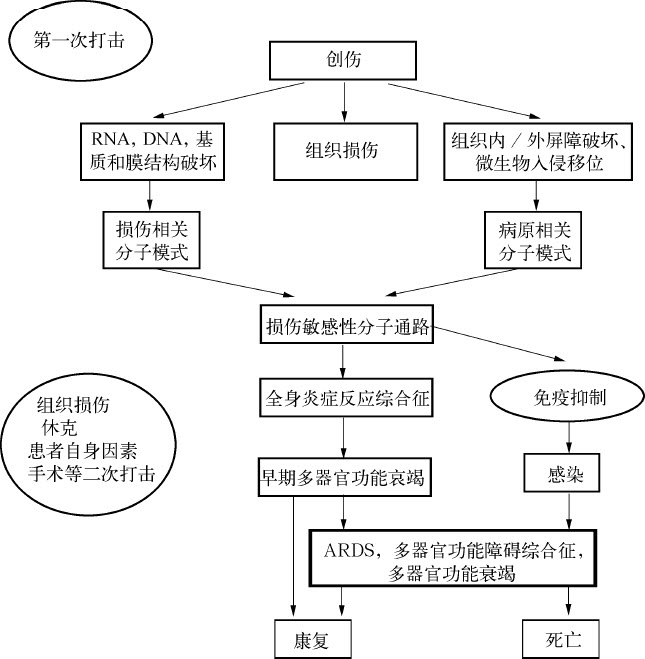
\includegraphics{./images/Image00140.jpg}
 \captionsetup{justification=centering}
 \caption{创伤通过分子通路导致炎症反应}
 \label{fig18-1}
  \end{figure} 

创伤刺激多种炎症介质以及相关多肽的释放,如单核细胞、巨噬细胞、T辅助细胞等可分泌白细胞介素-1、白介素-6、白介素-8、白介素-10以及肿瘤坏死因子等
\protect\hyperlink{text00024.htmlux5cux23ch12-23}{\textsuperscript{{[}12{]}}}
,在创伤患者炎症反应和多器官功能障碍发生过程中起重要作用。肿瘤坏死因子能导致巨噬细胞和自然杀伤细胞凋亡,刺激血栓素A\textsubscript{2}
、前列腺素、P选择素、血小板激活因子和细胞间粘附分子的表达。白介素-1是严重创伤患者中激活的另一个主要细胞因子,诱导T细胞和巨噬细胞活化,产生级联反应,激活多种炎症因子转录和表达。研究显示,白介素-6可作为创伤患者全身炎症反应综合征的诊断和有效预测并发症发生的指标
\protect\hyperlink{text00024.htmlux5cux23ch13-23}{\textsuperscript{{[}13{]}}}
,动物实验发现,阻断白介素-6至200pg/dl以下则可提高实验动物生存率。白介素-8是一种趋化因子,在创伤后的合成和分泌能动员淋巴细胞并在损伤区域得到活化。损伤后血浆白介素-8水平和ARDS及多器官功能衰竭发生的风险呈正相关,有研究显示,支气管肺泡灌洗液中白介素-8浓度和ARDS患者的死亡率呈正相关
\protect\hyperlink{text00024.htmlux5cux23ch14-23}{\textsuperscript{{[}14{]}}}
。白介素-10由淋巴细胞和单核细胞合成,主要作用是抑制单核巨噬细胞系统来源的TNF-α、白介素-6和白介素-8的活性。白介素-10作用于脂多糖刺激兔肺泡巨噬细胞,能减少参与ARDS过程炎性介质的合成。在针对脓毒性腹膜炎动物模型的研究中发现,白介素-10能提高其生存率,给予抗白介素-10的抗体能增加死亡率。损伤的内皮细胞产生的前列腺素和血栓素,以及组织胺和缓激肽等能进一步加重内皮细胞功能障碍和组织水肿,导致局部组织损伤,同时导致远隔器官功能障碍
\protect\hyperlink{text00024.htmlux5cux23ch12-23}{\textsuperscript{{[}12{]}}}
。

创伤的病理生理改变还受到多种因素的影响,研究显示性别因素和性激素在创伤患者免疫炎症反应中起了一定作用,有研究发现雄性动物在创伤失血后免疫炎症反应明显强于雌性动物
\protect\hyperlink{text00024.htmlux5cux23ch15-23}{\textsuperscript{{[}15{]}}}
。另外,临床研究还显示创伤患者炎症反应程度和并发症的发生率和患者基因型有关
\protect\hyperlink{text00024.htmlux5cux23ch16-23}{\textsuperscript{{[}16{]}}}
。

(4)严重创伤后免疫功能紊乱 从机体受到创伤开始直到愈合,整个病程的发生发展都与免疫系统功能状态密切相关。研究发现,严重创伤后发生免疫功能紊乱或失调,尤其是T淋巴细胞介导的细胞免疫功能受到显著的抑制,使免疫功能防御感染的能力明显减弱,导致机体感染、多器官功能衰竭的易感性增加。

神经内分泌激素对中枢和外周淋巴器的分泌功能和免疫细胞对外源抗原的反应及应答非常重要。下丘脑-垂体-肾上腺轴和下丘脑-垂体-甲状腺轴分泌产物可以直接或间接地影响淋巴细胞和免疫系统的上皮细胞,产生大量激素,如甲状腺素、胰高血糖素、糖皮质激素,导致免疫系统的激活。目前研究认为,创伤后巨噬细胞抗原提呈能力及活性因子分泌水平与应激状态下产生的具有免疫抑制作用的激素和神经肽释放增加有关,如糖皮质激素、促肾上腺皮质激素、雄激素、β内啡肽等。严重创伤后免疫应答存在着性别上的差异,女性比男性更能抵抗休克、创伤和脓毒血症诱导的免疫功能紊乱和器官损伤。

新近研究表明,炎症级联反应的激活在严重创伤后免疫功能紊乱的发生发展中起重要作用。巨噬细胞是炎症介质、活性氮介质、白介素-6、肿瘤坏死因子-α的主要来源,在免疫反应中扮演关键作用,可以上调或下调宿主的防御机制。严重创伤后巨噬细胞过度激活,导致致炎因子的释放大量增加,这在严重创伤后免疫功能紊乱的发生发展中起主要作用。严重创伤引起巨噬细胞功能改变,细胞因子(白介素-1、肿瘤坏死因子-α、白介素-6、转化生长因子-β)和前列腺素E\textsubscript{2}
合成增加,导致机体炎症介质水平显著升高
\protect\hyperlink{text00024.htmlux5cux23ch17-23}{\textsuperscript{{[}17{]}}}
。而巨噬细胞过度激活增加严重创伤后脓毒血症的易感性,因此Deitch提出了“二次打击”学说,严重创伤第一次打击主要是引起机体表现为异常反应(如炎症介质释放增加),二次打击(如感染)却可导致多器官功能衰竭和死亡
\protect\hyperlink{text00024.htmlux5cux23ch18-23}{\textsuperscript{{[}18{]}}}
。

T辅助细胞1/T辅助细胞2细胞因子在严重创伤后免疫功能紊乱中具有重要作用。T淋巴细胞是先天性免疫反应的一部分,其功能紊乱是严重创伤后免疫功能紊乱的诱发因素。严重创伤后免疫功能紊乱主要发生在T淋巴细胞介导的免疫,导致T辅助细胞1反应抑制,T辅助细胞2型细胞因子合成增加或不变。严重创伤后全身炎症反应综合征中细胞因子的合成也可能影响Th亚群的分布和随后的免疫反应。白介素-12具有很强的免疫调节特性,包括免疫细胞溶细胞活性的活化以及诱导T细胞和自然杀伤细胞合成干扰素-γ,有助于T辅助细胞反应,支持细胞介导免疫反应
\protect\hyperlink{text00024.htmlux5cux23ch19-23}{\textsuperscript{{[}19{]}}}
。白介素-12也能作为致炎细胞因子和免疫调节剂,调节先天性免疫和获得性免疫反应
\protect\hyperlink{text00024.htmlux5cux23ch20-23}{\textsuperscript{{[}20{]}}}
。

(5)多发性创伤患者易发生多器官功能障碍综合征 创伤早期反应主要是局部组织损伤(骨折、软组织损伤等)、早期直接的器官功能障碍(脑、肺等)以及疼痛等,并激活凝血系统和维持重要器官功能的反应。出血导致的休克,肺损伤导致的低氧、低血容量状态,脑损伤和低体温是早期威胁多发伤患者生命的主要问题。因此,创伤早期应特别关注这几种威胁患者生命的情况。早期准确的伤情评估和分类有助于给患者后续处理提供有益的指导,特别是面对一群多发伤患者的时候更为关键。还需要特别关注特殊人群,如青年人和运动员,其对休克的耐受能力强,可以在出现休克很长时间以后才出现血压的突然下降。

如创伤患者早期休克未能得到逆转,可能激活蛋白酶C途径
\protect\hyperlink{text00024.htmlux5cux23ch21-23}{\textsuperscript{{[}21{]}}}
,导致创伤性凝血病的发生。全身炎症反应导致的内皮细胞损伤进一步加重凝血功能障碍。约有1/4的多发性创伤患者随着创伤性凝血病的发生而出现低体温和酸中毒,这三种被称为死亡三角(lethal
triad),是创伤患者死亡的重要原因,故早期控制出血和防止热量丢失是防止死亡三角的关键
\protect\hyperlink{text00024.htmlux5cux23ch22-23}{\textsuperscript{{[}22{]}}}
。

多发性创伤患者各部位的创伤具有不同临床表现。头部创伤导致患者神经系统损害,出现神志改变,致残率和病死率高。面颈部创伤有出血窒息的危险。胸部创伤由于直接的肺损伤可导致创伤性湿肺、血气胸等导致低氧血症、呼吸困难、休克;直接心脏损伤等可导致患者短时间内死亡。腹部实质性脏器出血出现失血性休克,空腹脏器破裂导致腹膜炎。长骨骨折、骨盆骨折、腹膜后血肿患者休克发生率高,低血容量性休克多见。多发性创伤患者后期感染发生率高,多为混合感染。

多发性创伤患者在休克基础上合并感染、手术等二次打击,极易发生多器官功能障碍。多发性创伤患者遭受创伤打击后,激活先天性免疫和炎症反应,导致远隔器官损害,常常累及肺脏而出现急性呼吸衰竭,甚至ARDS。直接创伤导致肺实质细胞损伤,引起细胞结构和通透性的改变,此外,尚可通过激活补体途径和诱导细胞因子的产生而致肺内皮细胞损伤,微血管内皮细胞表面粘附分子的表达促进白细胞的粘附与聚集,对肺毛细血管、肺泡组织产生毒性作用,导致广泛微血栓形成、微循环障碍,出现肺水肿甚至肺功能不全。同时,内毒素可直接激活单核-巨噬细胞系统,合成、释放多种细胞因子(如肿瘤坏死因子-α、白介素-1等),作用于微血管内皮细胞,进一步加剧肺损害。近年来也有研究发现,胃肠道功能在早期就受损,胃肠道是全身最大的细菌和内毒素库,肠屏障功能受损可引起肠道细菌移位和门静脉内毒素血症,从而激活肝脏单核-巨噬细胞系统,启动全身炎症反应。随着病情进展,常可相继出现肝肾衰竭,而心血管或血液系统衰竭通常是多器官功能障碍综合征的终末表现。

\subsubsection{多发性创伤的诊治}

(1)多发性创伤的救治模式 在多发性创伤的急诊救治中,需改变常规的诊疗模式,由原来诊断→治疗模式转变为抢救→诊断→治疗模式。详细的诊断和确定性治疗必须是抢救工作获得一定成效后再进行,决不能因诊断而延误抢救时机。伤后60分钟是决定患者生死的关键时段,属危重症抢救阶段,被称为抢救的“黄金时间”,即“黄金1小时”。多发性创伤救治应及时而准确地全面估计伤情,有全局、整体观念,及时处理危及患者生命的器官损伤,要突出“快、准、及时、高效”的急救原则。

多发性创伤患者死亡有3个高峰期:①伤后数秒至数分钟内,多因颅脑、高位脊髓、心脏或大血管损伤而立即死亡;②伤后数分钟至数小时内,多因窒息、呼吸循环功能不全、未能控制的大出血而早期死亡;③伤后数天至数周内,因器官功能衰竭或感染等而晚期死亡。因此,完善的院前急救和急救网络系统的快速反应是提高多发性创伤患者生存率的首要条件。

(2)多发性创伤的现场抢救 多发性创伤患者的有效救治须从受伤现场开始,但不可把现场急救的目标定得过高。在救治条件好的城市或郊区,现场急救的任务应限定为:发现危重患者并将其移离险恶环境,进行最初步的紧急处理,如清除阻塞气道的口咽部异物、加压包扎制止外出血、肢体骨折的简单固定、建立静脉通道以便运转途中输液等,以上操作应在10分钟内完成。迅速将患者运送到有条件的医疗机构,最好是创伤急救中心。

临床研究证实,在现场进行过多的急救治疗不但可能无益,而且可能是有害的,时间上的任何拖延都会增加死亡发生的风险,影响患者的预后。而在救治条件较差的边远地区,或同一时间有大批患者不可能立即全部转运时,则须就地进行较长时间的救护。

(3)多发性创伤的急诊抢救 患者送抵医院(急诊室或创伤中心)后,即由接诊医师迅速进行概要的检查。在伴有休克或呼吸功能障碍的危重患者,收集病史及查体应与复苏同步进行,目的是尽快查明危及生命的严重损伤。诊断要求快、准,尽量少搬动,并应在最短时间内明确脑、胸、腹部是否有致命性的损伤。

近年来,多发性创伤的诊断技术虽有进步,但在急诊情况下,仔细、准确和反复的检查仍是判明伤情的重要手段。危重患者的衣服必须全部去除以保证充分暴露,但要注意保暖。首先是查明有无对患者生命构成迫在眉睫的威胁、需要立即处理的伤情,如果有气道阻塞、张力性气胸、开放性气胸等,必须及时解决,否则患者将很快死亡;其次,休克复苏、控制明显的外出血和解除可能导致脑疝发生的颅内高压也是需要完成的紧急任务。

积极的液体疗法恢复有效血容量是复苏的关键环节,但对于严重胸、腹部创伤患者,内出血尚未得到控制之前,并不主张“充分”输液和快速提升血压至正常水平,以免加重出血和血液过度稀释(血红蛋白<70g/L或血细胞比容<0.20)。将收缩压暂时维持在满足重要脏器灌注的水平,手术止血后再按需要扩充血容量,可以降低死亡率,延长生存时间,这就是所谓“限制性复苏”。待生命体征初步稳定后,应对患者按系统进行全面检查。必要的辅助检查也应在此时进行,如X线摄片、头颅和躯干CT、腹部B超等,但仍以少搬动患者为原则。

(4)多发性创伤手术时机与方式的选择 严重多发性创伤的处理重点和先后顺序十分重要。应区别轻重缓急,优先处理危及生命的损伤。颅脑、胸、腹部损伤是处理的重点。广泛脑挫裂伤、颅内血肿应迅速开颅减压。同时伴胸腔或腹腔大出血者,开颅应与开胸或开腹同时进行。胸部、腹部同时受伤,可根据严重程度确定先后顺序。胸部重伤者先开胸;腹部伤重者做胸腔闭式引流后先开腹,胸部、腹部伤均很严重时,应同时分别开胸和开腹,尽量避免做胸腹联合切口。不累及大血管的肢体骨折,有条件者可以在颅脑、胸、腹创伤处理后及时手术固定,但若伤情危重,则应待患者病情进一步稳定后再处理。

对于严重创伤患者,应依据损伤控制性手术治疗原则进行救治。特别严重的多发性创伤,常表现为顽固性低体温(<35℃)、顽固性代谢性酸中毒(pH<7.30,血乳酸>5mmol/L)和凝血障碍(凝血酶原时间或部分凝血活酶时间超过正常的50%),统称为“死亡三角”。此类患者多不能耐受常规的确定性手术治疗,必须给予特殊的处理,把手术目标局限在控制创伤损害上,根据损伤控制外科(damage
control surgery)的原则施行“损伤控制性手术”(damage control
operation),目的是挽救生命;主要任务是通过最简单快捷的方法止血(填塞或缝合)和控制污染源(破裂肠管外置、缝合,不做吻合),迅速结束手术,送重症医学科进一步复苏,病情稳定后再行确定性手术
\protect\hyperlink{text00024.htmlux5cux23ch5-23}{\textsuperscript{{[}5{]}}}
。

(5)多发性创伤的后期救治 在多发性创伤救治全过程中,早期是抢救生命、复苏,中期是确定性手术、防治多器官功能衰竭和感染,后期是矫正、治疗各种后遗症和畸形,并康复
\protect\hyperlink{text00024.htmlux5cux23ch2-23}{\textsuperscript{{[}2{]}}}
。此3阶段是紧密相连的,救治的每一步骤都要想到下一步可能会出现的问题并予以预防,如休克期复苏要防止灌注不足导致肾衰竭等多脏器功能障碍,因而要快速输液提升血压,防止低血压时间过长;大量输液抗休克又要防止输液过量引起肺水肿、ARDS、脑水肿和腹腔间隔室综合征等。

进行抢救手术前、术中都要注意无菌操作,预防感染,防治DIC等。术后定期测定血(尿)电解质变化、血常规、肝肾功能、凝血和纤溶功能,必要时做血培养和可疑感染部位的涂片和培养,根据检查结果,调整输液种类和输液量,必要时改变抗生素的种类和剂量。长期卧床者还须防治深静脉血栓、急性肺栓塞。在不能经口服或口服营养不足时,应静脉补充氨基酸、脂肪乳剂、各种维生素和微量元素。禁食较长时间者,早期应用全胃肠外营养。

严重多发性创伤救治的时效性与整体性两大专科特色是提高创伤救治水平的根本保证
\protect\hyperlink{text00024.htmlux5cux23ch5-23}{\textsuperscript{{[}5{]}}}
\textsuperscript{,}
\protect\hyperlink{text00024.htmlux5cux23ch23-23}{\textsuperscript{{[}23{]}}}
\textsuperscript{,}
\protect\hyperlink{text00024.htmlux5cux23ch24-23}{\textsuperscript{{[}24{]}}}
,创伤专业化、重症医学科的加强监护和快速、整体化治疗模式可明显提高多发性创伤救治的成功率
\protect\hyperlink{text00024.htmlux5cux23ch25-23}{\textsuperscript{{[}25{]}}}
,提高多发性创伤的救治水平。

多发性创伤的诊治要点是先抢救生命,边诊断、边治疗,必须有动态、整体观念,高度重视应激导致的炎症反应和免疫抑制,加强营养支持,预防感染等二次打击,防治器官功能衰竭。另外,建立创伤急救新模式是未来我国多发性创伤救治的必要条件,加强急救复合型人才和创伤专业化人才培养是关键,创立区域化、多功能的创伤治疗中心是未来我国创伤救治的趋势。

\section{临床问题}

\subsection{失血性休克的紧急处理和复苏}

\subsubsection{早期失血性休克有哪些处理原则?何谓治疗的黄金时间?}

早期失血性休克的治疗是以救命为主,采取先救治、后诊断或边救治、边检查诊断的方式进行抗休克治疗,其程序是保证呼吸道通畅及保证通气(ventilation)、补液及输血扩充血容量(infusion)、监测心泵功能(pulsation)、紧急控制出血(control
bleeding),这4个步骤被称为VIPC计划。也可将失血性休克的早期救治概括为ABCD阶段:首先保持呼吸道通畅(airway)及充分供氧(breath);液体复苏(circulation),保证脏器灌注;紧急控制出血,尽早手术止血或应用介入、微创等手段止血,积极进行脏器功能支持,防治多器官功能障碍(dysfunction)。

多发创伤、骨折、脏器破裂、血管损伤引起的难以控制的大出血,患者多在伤后1~2小时内死亡,因此,应抓紧伤后1小时的“黄金时间”进行救治,做到迅速、准确、及时而有效。伤后1小时的“黄金时间”内,头10分钟是决定性的时间,被称为“白金10分钟”,这段时间内如果患者的出血被控制,并能预防窒息、缺氧的发生,则可避免患者早期死亡。“白金10分钟”期间的抢救应以避免发生心脏骤停为目标,为后续的抢救赢得时间。

\subsubsection{什么情况下失血性休克需实施限制性液体复苏?有何临床意义?}

传统的抢救创伤失血性休克的治疗原则是在处置创伤的同时,尽快、尽早地经静脉大量补充液体进行复苏,其目的是迅速恢复有效循环血量,使生命体征尽可能恢复或接近正常,并维持重要器官的血液灌注。但目前越来越多的报道表明,出血未控制的创伤失血性休克,早期大量液体复苏虽然可以将血压提升上来,但是会带来严重的副作用
\protect\hyperlink{text00024.htmlux5cux23ch26-23}{\textsuperscript{{[}26{]}}}
。因为出血未控制,血液的过度稀释会引起稀释性凝血功能障碍,不易形成新的凝血块或者使已形成的凝血块脱落,易加重出血或引发再出血;血液过度稀释,血红蛋白浓度降低,不利于氧的携带和运送,会减少组织氧供而引起代谢性酸中毒;大量补液会造成肺水肿、肺间质水肿,不利于氧的弥散。因此,提出了限制性液体复苏(limited
fluid resuscitation)的概念。

限制性液体复苏适用于有活动性出血的休克患者,尤其适用于胸部和腹部创伤为主的有活动性出血的休克患者。快速的大量补液极有可能使心脏和胸腹部已经凝聚的血块脱落,造成危及生命的再次大出血,丧失手术时机。对肺部挫伤适当限液会减少肺水肿发生和减轻严重程度。如果到达创伤中心的时间比较长,应尽可能简单有效地处理明显的外出血,适当扩容、维持收缩压在90mmHg以上,保证重要脏器灌注,尽早有效止血。但是对于合并颅脑外伤的严重休克患者,当务之急是立即颅脑手术清创,彻底止血、充分减压。但需明确的是,平均动脉压不可降得太低,否则会影响脑的灌注,同时也不可过高,以免加重脑水肿和出血。

限制性液体复苏是近年来研究的一个热点,即在进行手术控制出血前,谨慎实施限制性液体措施,避免血压过高、血液过度稀释,以减少内出血,其目的是寻求一个复苏平衡点,既可以通过液体复苏适当地恢复组织器官的血液灌注,又不至于过多地扰乱机体的代偿机制和内环境。动物实验及临床研究结果表明,限制性液体复苏对于非控制性出血休克效果优于积极复苏(aggressive
resuscitation)
\protect\hyperlink{text00024.htmlux5cux23ch27-23}{\textsuperscript{{[}27{]}}}
。但限制性复苏具体控制多高血压、维持多少时间,尚需进一步确证。有学者认为若没有合并颅脑损伤,收缩压可控制在90mmHg,若合并颅脑损伤,为保证脑组织有足够血液灌注,收缩压应维持在100mmHg以上。

为了保证脏器灌注,防止器官功能障碍,应尽快采取控制出血的措施,尽量缩短限制性液体复苏的持续时间,有效处理后尽快进行积极的液体复苏。

\subsubsection{失血性休克延迟复苏适用于哪些患者?有何临床意义?}

传统观点认为,创伤休克应立即进行液体复苏,使用血管活性药物,尽快提升血压。但如今的观点对有活动性出血的创伤失血性休克患者,不主张给予快速大量的液体进行即刻复苏和使用血管活性药物尽快提高血压,而主张在彻底止血前,只给予适量的液体维持机体基本需要,在手术彻底处理后再进行充分的复苏,即所谓的延迟复苏(delayed
fluid
resuscitation)。过早地使用血管活性药物或输注大量液体提升血压,并不能提高患者的存活率,反而有增加死亡率和并发症的危险
\protect\hyperlink{text00024.htmlux5cux23ch28-23}{\textsuperscript{{[}28{]}}}
。

Bickell等观察了液体延迟复苏与即刻复苏(immediate
resuscitation)治疗589例失血性休克患者的疗效,其中延迟复苏289例,即刻复苏309例,结果表明即刻复苏组和延迟复苏组在术前的血压基本相同,但即刻复苏组平均输液量是延迟复苏组的7倍,而延迟复苏组的各项生理指标,如血红蛋白含量、凝血酶原时间、部分凝血活酶时间、动脉血pH、术后并发症(如急性肾衰竭、ARDS等)发生率及患者病死率均较优
\protect\hyperlink{text00024.htmlux5cux23ch29-23}{\textsuperscript{{[}29{]}}}
。目前液体延迟复苏策略在失血性休克治疗中的地位越来越受到重视。

对于伴有活动性出血的失血性休克患者可以考虑延迟复苏,但延迟复苏并不是不复苏,应密切观察患者的病情变化,给予适量的液体进行控制性复苏,同时应积极控制出血,尽可能早地予以充分复苏。

\subsubsection{早期失血性休克选用什么液体进行复苏?}

液体复苏是创伤失血性休克治疗的重要环节,复苏治疗是否及时有效,直接影响患者的最终生存。复苏液体通常分为晶体液和胶体液,晶体液又分为等渗液和高渗盐液,胶体液有白蛋白、血液和血液代用品、右旋糖酐、明胶和羟乙基淀粉等。关于复苏液体的选择近年来一直存在争议。

平衡盐为最常用的复苏液体之一,其电解质成分和渗透压与血浆相仿,输入后还可以补充丧失的功能性细胞外液、降低毛细血管内血黏度、改善微循环灌流,但输入后仅有25%~30%存留在血管内,大部分液体将转移至细胞内及组织间隙,大量应用时可增加组织水肿,特别是肺水肿的机会。研究表明,等渗晶体尤其是乳酸林格液具有显著的激活免疫反应(主要为中性粒细胞)及诱导细胞损伤作用,使休克患者因炎症反应诱发的晚期并发症发生率增加。因此建议应适量应用等渗晶体液。

高渗晶体液能快速升高血压、增加心排血量、改善循环功能,同时还具有对心、肺功能干扰小和不增加颅内压、用量小等优点。作用机制是通过渗透压的作用吸引水分进入循环而扩充血容量。与等渗晶体液相比,高渗晶体液还具有抑制中性粒细胞引起的免疫反应及细胞损伤较少的特点。其与胶体合用不失为一种较理想的复苏手段。近年来,许多研究者应用7.5%的高渗NaCl和6%羟乙基淀粉抢救创伤失血性休克患者收到良好效果。

与晶体液比较,人工胶体液如6%羟乙基淀粉和琥珀酰明胶,具有扩容效果显著及维持时间相对较长的特点,且到达复苏终点所需输入液体量少,但需警惕对患者肾功能和凝血功能的影响。

全血和成分输血是严重失血性休克不可缺少的复苏液体,但有价格昂贵、来源有限或有感染血源性传染病的风险等缺点。

就复苏液体种类而言,晶体还是胶体,晶体液中选择高渗溶液还是低渗溶液,目前尚无统一认识。2004年发表的SAFE
study入选了16个重症医学科的近7000例患者,随机采用4%白蛋白和生理盐水进行液体复苏,显示两组28天病死率、重症医学科及住院时间、机械通气时间、肾脏替代治疗时间均无明显差异。亚组分析显示,对于合并颅脑损伤的创伤患者,白蛋白组的病死率高于生理盐水组(相对危险度为1.62),其他创伤和非创伤患者两组间无明显差异,但颅脑损伤的两组病例白蛋白组241例死亡59例,生理盐水组251例死亡38例,白蛋白组患者病死率风险明显增加
\protect\hyperlink{text00024.htmlux5cux23ch30-23}{\textsuperscript{{[}30{]}}}
。有学者提出以平衡盐液为首选液体,因为无论其电解质成分,还是渗透压均接近正常人的体液,还可以补充丧失的功能性细胞外液。但需注意的是,单独应用晶体溶液对改善血液动力学效果较差,且维持时间短、用量大,故必要时应补充一定量胶体溶液(通常主张晶∶胶体为2~3∶1)。

\subsection{多发性创伤的抢救流程和损伤控制外科}

\subsubsection{多发性创伤的诊断标准是什么?}

多发性创伤的诊断标准
\protect\hyperlink{text00024.htmlux5cux23ch23-23}{\textsuperscript{{[}23{]}}}
见表\ref{tab18-1}。\footnote{*表中有2项或2项以上合并存在时,即为多发性创伤;但仅有上肢和下肢骨折合并者,为多发性骨折,不诊断为多发性创伤。}

\begin{table}[htbp]
\centering
\caption{多发性创伤的诊断标准\textsuperscript{*}}
\label{tab18-1}
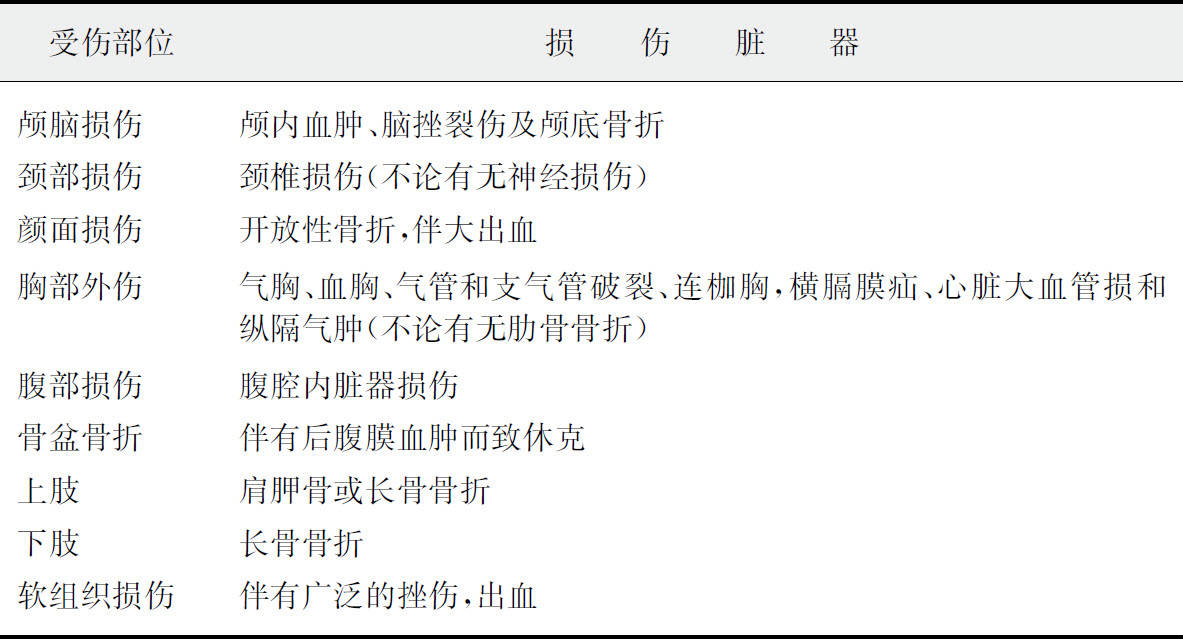
\includegraphics{./images/Image00141.jpg}
\end{table}

\subsubsection{严重多发性创伤应遵循的抢救检查要点是什么?}

多发性创伤危重患者到达急诊科后,就诊医生首先应注意患者的神志、面色、呼吸、血压、脉搏、体位、出血、伤肢姿态,有无大小便失禁、衣服撕裂和血迹、呕吐物的性状等情况。这些征象可反映患者的全身情况及有无危及生命的致命伤。尤其应注意患者有无呼吸道梗阻、心跳呼吸骤停、休克、大出血等致命征象。

对危重患者接诊后,应立即脱去衣物,迅速进行全身检查,主要检查呼吸道是否畅通、有否出血、有否休克等。为了不至遗漏重要伤情,建议急诊医生应牢记“CRASH
PLAN”以指导检查,以便尽可能达到不漏诊。C=心脏(cardiac),R=呼吸(respiration),A=腹部(abdomen),S=脊柱脊髓(spine),H=头颅(head),P=骨盆(pelvis),L=四肢(limb),A=动脉(arteries),N=神经(nerves)
\protect\hyperlink{text00024.htmlux5cux23ch31-23}{\textsuperscript{{[}31{]}}}
。

实验室检查与特殊检查项目包括:查血型和交叉配血、动脉血气分析、测定血红蛋白含量、血细胞比容、白细胞计数、肝功能、电解质、血糖、血尿素氮和肌酐及尿常规。如患者伤情稳定,可及时行心电图、X线、B超、CT等检查。对伤情不稳定的患者,可进行床旁心电图、床旁X线摄片、床旁B超等检查。

某些隐蔽的深部损伤初期临床表现常不明显。必须反复检查、动态观察。再次检查的重点包括腹膜后十二指肠破裂、胰、肾、部分结肠损伤以及有无延迟性腹内、胸内、颅内出血和迟发的气胸等。

\subsubsection{多发性创伤急诊检查的注意事项是什么?}

多发性创伤患者到达急诊后应注意:

(1)发现危重情况如窒息、大出血等,必须立即抢救,不能单纯为了检查而耽误抢救时机。

(2)检查步骤尽量简捷,询问病史和体格检查可同时进行。检查动作必须谨慎轻巧,切勿因检查而加重损伤。

(3)重视症状明显的部位,同时应仔细寻找比较隐蔽的损伤(如肋骨骨折合并肝、脾破裂)。

(4)接收批量伤员时,不可忽视异常安静的病人。因为有窒息、深度休克或昏迷者已不能呼唤呻吟。

(5)一时难以诊断清楚的损伤,应在对症处理过程中密切观察,可采用B超等无创或微创手段,争取尽早确诊。

\subsubsection{何谓VIPC?}

严重多发性创伤抢救的程序可归纳为VIPC:

(1)V=ventilation 要求保持呼吸道通畅并充分通气供氧。在处理多发性创伤患者特别是头、颈、胸部伤患者时,首先应保持呼吸道畅。对颅脑外伤者,及时清除口腔血块、呕吐物、痰及分泌物,必要时做气管内插管,用呼吸机进行机械通气。对颌面外伤、颈椎外伤、喉部外伤,应早期行经皮穿刺气管切开套管置入术或气管切开术。

(2)I=infusion 指输液、输血扩充血容量及细胞外液。多发性创伤休克主要的病理变化是有效血容量不足,微循环障碍。因此,在抢救严重多发性创伤患者时,恢复血容量的重要性不亚于纠正缺氧。但Buris等提出了延迟(限制性)液体复苏的概念,即对创伤失血性休克,特别是活动性出血患者,不主张快速给予大量的液体复苏,而主张手术彻底止血前,给予少量平衡盐液,维持机体基本需要,手术止血之后再根据血流动力学和氧代谢监测进行复苏
\protect\hyperlink{text00024.htmlux5cux23ch32-23}{\textsuperscript{{[}32{]}}}
。

(3)P=pulsation 指对心泵功能的监测。多发性创伤患者的休克除低血容量休克和创伤性休克外,亦要考虑到心源性休克,特别伴有胸部外伤的多发性创伤,可因心肌挫伤、心脏压塞、心肌梗死或冠状动脉气栓而致心泵衰竭。有时低血容量性休克、创伤性休克和心源性休克可同时存在,故在严重多发性创伤抢救中要监测心电图及必要的血液动力学的变化,如中心静脉压、平均动脉压和心输出量等。

(4)C=control
bleeding 是指在多发性创伤抢救中紧急控制明显或隐蔽性出血。多发性创伤应边抢救抗休克、边完善相关检查、明确各处损伤的严重程度,尽早行损伤控制手术,颅脑、胸、腹部创伤是处理的重点,解决危及生命的出血和其他损伤,如颅内高压等,之后进入重症医学科严密监护和防治多器官功能障碍综合征,病情稳定后再行确定性手术,改善损伤脏器功能,以及康复治疗。

\subsubsection{何谓损伤控制外科?有何临床意义?}

损伤控制外科(damage control
surgery)是近20年来创伤外科领域中涌现出来的极有实用价值的外科概念,包括采用简便可行、有效而损伤较小的应急救命手术处理致命性创伤,进一步复苏和计划分期手术处理非致命性创伤的处理模式。“损伤控制”(damage
control)一词最早源于美国海军,意思是指一艘轮船承受损害和维持完整性的能力。损伤控制外科的3阶段原则为:初始简化手术、复苏和确定性手术。损伤控制外科的目的是救命、控制污染、避免发生多器官功能障碍综合征、为计划确定性手术赢得时机。1983年,Stone等对17例严重创伤患者采用早期简化手术、复苏和再次确定性手术,结果12例存活,而对照组14例患者采用常规治疗、详尽手术、关闭腹腔并行引流的患者中仅存活了1例
\protect\hyperlink{text00024.htmlux5cux23ch33-23}{\textsuperscript{{[}33{]}}}
。损伤控制外科的合理应用可以降低严重创伤患者的病死率
\protect\hyperlink{text00024.htmlux5cux23ch34-23}{\textsuperscript{{[}34{]}}}
。

损伤控制外科的具体内容包括:①立即手术,用最简单的方法控制出血和污染;②重症医学科的加强监护治疗,包括复苏、纠正低温、纠正凝血障碍和酸中毒,呼吸支持,防治多器官功能障碍综合征;③当患者病情允许时实施确定性手术
\protect\hyperlink{text00024.htmlux5cux23ch35-23}{\textsuperscript{{[}35{]}}}
。

损伤控制外科最初成功运用于严重腹部创伤的患者,随着外科技术的不断发展和进步,也适用于胸心外科、血管外科、泌尿外科等,需要实施损伤控制外科的适应证为:①损伤严重,如高能量的腹部钝器伤、多发性腹部穿透伤,合并低血流动力状态(包括低血压、心动过速、心动过缓、精神状态的改变等)、凝血障碍和(或)低体温。②合并复杂损伤,如重要的腹部血管损伤合并多发内脏损伤、多灶或多腔隙出血并内脏损伤、需要优先处理的多部位严重损伤。③其他主要因素,如严重的代谢性酸中毒、动脉血pH<7.30、低体温<35℃、复苏和手术时间>90分钟、非出血性原因引起的凝血障碍和大量的输液(红细胞>10U)。

研究发现,多发性创伤尤其是并发胸、腹部损伤者,伴有股骨干骨折时,宜先做简单的外固定,而将确定性的骨折固定手术(如髓内钉固定等)延至患者全身情况稳定后,可降低术后并发多器官功能障碍综合征的危险性,降低病死率
\protect\hyperlink{text00024.htmlux5cux23ch17-23}{\textsuperscript{{[}17{]}}}
。

\subsection{重度颅脑外伤的诊断及治疗}

\subsubsection{颅脑外伤的严重程度分级标准是什么?}

颅脑外伤常采用的严重程度分级标准为:

(1)轻型(指单纯性脑震荡伴有或无颅骨的骨折) ①昏迷0~30分钟;②仅有轻度头晕、头痛等自觉症状;③神经系统和脑脊液检查无明显改变。

(2)中型(指轻度脑挫裂伤伴有或无颅骨骨折及蛛脑膜下腔出血,无脑受压者) ①昏迷12小时以内;②有轻度神经系统阳性体征;③体温、脉搏、呼吸有轻度变化。

(3)重型(指广泛颅骨骨折,广泛脑挫裂伤及脑干损伤或颅内出血) ①深昏迷,昏迷12小时以上,意识障碍逐渐加重或出现再昏迷;②有明显神经系统阳性体征;③体温、呼吸、脉搏、血压有明显改变。

(4)特重型(指重型中更重者) ①严重原发性脑损伤,伤后深昏迷,有去大脑强直或伴有其他部位的脏器伤、休克等;②已有晚期脑疝表现,包括双瞳散大,生命体征严重紊乱或呼吸已停止。

此外,还可按Glasgow昏迷评分(GCS)(表\ref{tab18-2})评价颅脑外伤的严重程度:①轻型:GCS评分13~15分,伤后昏迷在30分钟内;②中型:GCS评分9~12分,伤后昏迷30分钟至6小时;③重型:GCS评分3~8分,伤后昏迷6小时以上,或在伤后24小时内病情恶化再次昏迷6小时以上者,其中GCS评分3~5分者可列为特重型。

\begin{table}[htbp]
\centering
\caption{Glasgow昏迷评分}
\label{tab18-2}
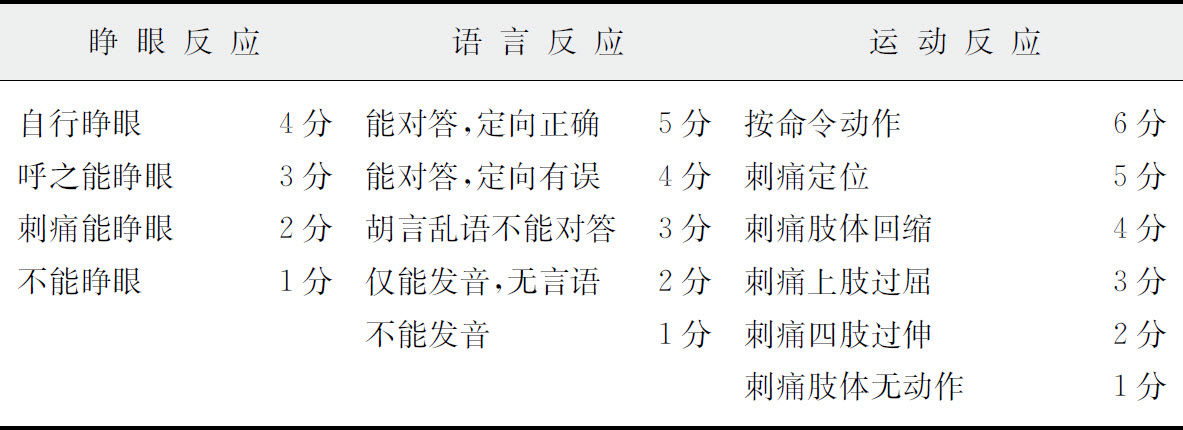
\includegraphics{./images/Image00142.jpg}
\end{table}

\subsubsection{监测颅内压的方法有哪些?有何临床意义?}

重度颅脑外伤后颅内压监测指征可根据昏迷程度来判断,Glasgow昏迷评分法(GCS)≤8分时需要颅内压监测和重症医学科监护。有潜在病情变化的轻中型颅脑外伤(GCS评分9~15分)、CT复查有血肿增大但尚不需手术、伤后有休克及低氧血症等有颅内压增高趋势的也是颅内压监测指征。

目前国内对颅内压评估主要靠临床表现、CT、腰穿监测脑脊液压力和颅内压直接测量来判断,而国际上公认的是放置颅内压监测器进行有效监测,根据颅内压监测指导治疗,可能降低严重颅脑外伤患者的病死率,改善预后。

目前常用的监测方法包括
\protect\hyperlink{text00024.htmlux5cux23ch36-23}{\textsuperscript{{[}36{]}}}
:

(1)脑室内导管法 常用一根光纤导管放入脑室内,与床边压力传感器相连,传感器须位于Monroe孔(外耳道)水平以此为参考点,导管由三通阀与压力传感器外引流系统相连,可持续监测颅内压。该方法优点是准确,且可以排放脑脊液降低颅内压力,但容易感染。

(2)脑实质内光纤传感器 通过直径4mm中空导管,一条细纤维光缆经颅骨入脑实质内,一般置入脑实质内的非功能区(如右额叶等),经与纤维光缆顶端与压力传感器相连,可随压力变化产生光传导信号,信号经纤维光缆传出可计算颅内压。该方法感染率低,但也有缺点,如排放脑脊液需另置引流导管。

(3)蛛网膜下腔导管 头颅钻孔后放入中空导管,基底部用腰穿针刺破,使脑脊液充满导管,再将压力管道系统与压力传感器相连。该方法优点是感染率低,但误差大,导管容易脱落或破碎屑堵塞,目前国外已不再使用。

(4)硬膜外传感器 置于硬膜表面,通过光学传感器传导压力,由于硬脑膜完整,颅内感染发生率低,但准确性稍差。

以上这些颅内压监测法,都有创伤性,导管易损坏,同时容易引起颅内感染,因此使用需严格无菌,按操作规程操作。

目前国内外尚缺乏理想的非创伤性颅内压监测技术进行正确和连续测量。超声多普勒为非创伤性检测技术,通过超声测定颅底动脉血流速度估计颅内压,当颅内压升高时,可见舒张期血流减慢,收缩期血流峰变陡,搏动指数增高等。当颅内压力达到舒张期血压时,可见舒张期血流消失。还有采用外耳道声阻抗法测定放射声音,以检测鼓膜传导回声来评估颅内压力改变,但因颅内压增加时可导致卵圆窗压力增加,故该技术尚在研究阶段。

\subsubsection{动态CT检查在重度颅脑外伤诊治中有何临床意义?}

部分颅脑外伤患者原发颅脑损伤并不重,但在病程中出现严重的继发性损伤,而伤后72小时内是迟发性外伤性脑内血肿形成的高峰(72.4%~93.1%),因此在伤后72小时内应密切观察病情变化,如意识、瞳孔、神经系统体征、生命体征等,必要时复查CT,任何时候的神经系统体征和功能改变均需要立即复查CT。条件许可的可行动态CT扫描检查。

动态CT检查可早期发现迟发性血肿,了解脑水肿范围、程度,脑室有无受压等重要情况,有助于非手术治疗过程中或手术后确定疗效、更改治疗方案,以及时处理并发症。

复查CT指征包括:①意识障碍无明显好转甚至逐渐加重;②血肿清除后一度好转后又逐渐加重;③颅内压监测提示颅内压持续增高;④神经系统出现新的阳性体征,特别是一侧瞳孔散大、甚至出现急性脑疝征象;⑤对冲性脑挫裂伤或者减速性脑损伤,经保守治疗无明显好转甚至逐渐加重。

\subsubsection{闭合性重度颅脑外伤的手术治疗原则是什么?}

对于幕上20~30ml的血肿、无明显颅内压增高症状或轻微中线移位、脑池或脑室无受压者,可保守治疗;血肿较大或颅内压明显增高者须早期手术。

颅内血肿的手术指征为:①意识障碍程度逐渐加深;②颅内压的监测压力超过270mmH\textsubscript{2}
O,并呈进行性升高;③有局灶性脑损害体征;④尚无明显意识障碍或颅内压增高症状,但CT检查血肿较大(幕上者>40ml,幕下者>10ml),或中线结构移位明显(移位>1cm)、脑室或脑池受压明显;⑤在非手术治疗过程中病情恶化者。

硬脑膜外血肿因不易吸收,故应放宽手术指征。

重度脑挫裂伤合并脑水肿的手术指征为:①意识障碍进行性加重或已有一侧瞳孔散大的脑疝表现;②CT检查发现中线结构明显移位、脑室明显受压;③在脱水、激素等治疗过程中病情恶化者。

重型颅脑损伤开颅术经过几十年的实践与探索,已经形成一套标准的术式。采用标准大骨瓣开颅术能清除约95%单侧幕上颅内血肿,其余5%幕上顶后叶、枕叶及颅后窝血肿则需行其他骨瓣开颅术。

\subsubsection{重度颅脑外伤综合治疗措施有哪些?}

重度颅脑外伤除了严密观察病情、及时有效的手术治疗外,还需要采取以下综合治疗措施。

(1)改善脑血流、避免脑缺血缺氧 这是维持脑组织正常代谢的基本条件。脑灌注压和脑血流量下降是造成神经组织缺血性损伤的根本原因,尽可能避免任何时候的低血压和低氧状态发生,合适的氧合,适当的液体复苏,维持脑灌注压在70mmHg以上。

(2)降颅内压治疗 甘露醇为渗透性利尿剂,研究显示间歇给药治疗较持续灌注更有效,有效剂量为0.25~1g/kg。应补充适量液体维持正常的血容量。甘露醇与呋塞米(速尿)交替使用效果较好。另外应早期防治脑血管痉挛、改善脑血流量,从病因上加以治疗。伴有肾功能损害者可换用甘油果糖或白蛋白加呋塞米行脱水治疗。但已经有研究显示,大剂量长期使用白蛋白对颅脑外伤患者是有害的
\protect\hyperlink{text00024.htmlux5cux23ch37-23}{\textsuperscript{{[}37{]}}}
,但可常规剂量间断使用。

(3)亚低温 重型颅脑损伤患者应用亚低温治疗后,颅内压明显下降,疗效明显优于正常体温组。亚低温对重型颅脑损伤保护作用机制有:①降低脑组织氧耗量,减少乳酸堆积;②保护血脑屏障,减轻脑水肿;③抑制兴奋性氨基酸、自由基及一氧化氮等有害物质释放,减少对脑组织损害;④减少钙离子内流,阻断钙对神经元的毒性作用;⑤减少脑细胞结构蛋白破坏,促进脑细胞结构和功能修复。

(4)营养支持疗法 重型颅脑损伤患者全身代谢紊乱,主要表现为基础代谢率升高、能量消耗增加、蛋白质分解利用大于合成,以及负氮平衡状态、低蛋白血症和高糖血症。严重全身代谢紊乱会引起或加重继发性脑损害,从而增加重型颅脑损伤的致残率和病死率。营养补充的途径有胃肠内营养和胃肠外营养。

(5)激素 糖皮质激素曾广泛应用于重型颅脑损伤患者,近年来大多数临床研究结果令人失望。2004年英国《柳叶刀》杂志发表关于大剂量糖皮质激素治疗10008例急性颅脑损伤患者的前瞻性、随机、双盲临床对照研究结果,5007例急性颅脑损伤患者(Glasgow昏迷评分<14分)伤后8小时内给予大剂量甲基强的松龙治疗(48小时甲基强的松龙总剂量21.2g),另5001例同样伤情患者给予安慰剂作为对照组,结果表明甲基强的松龙组患者死亡率21.1%,对照组死亡率为17.9%,可见糖皮质激素显著增加了患者病死率(\emph{P}
=0.0001),而导致死亡率增加的主要原因是感染和消化道出血
\protect\hyperlink{text00024.htmlux5cux23ch38-23}{\textsuperscript{{[}38{]}}}
。有关常规剂量糖皮质激素治疗急性颅脑创伤患者的疗效争议很大,现尚无确切结论。目前认为,对于颅脑损伤患者,不应该常规使用大剂量糖皮质激素,更不能大量或长期滥用激素
\protect\hyperlink{text00024.htmlux5cux23ch39-23}{\textsuperscript{{[}39{]}}}
。但对气管插管的多发性创伤患者早期应用应激剂量糖皮质激素可以降低院内获得性肺炎的发生率
\protect\hyperlink{text00024.htmlux5cux23ch40-23}{\textsuperscript{{[}40{]}}}
。

(6)钙拮抗剂 严重急性颅脑创伤患者不提倡使用。对于无明显颅内高压的外伤性蛛网膜下腔出血患者,由于大量血液进入蛛网膜下腔以及血液崩解产物的刺激,使脑血管发生痉挛,加重脑损伤,因此可适当使用。早期及时应用钙拮抗剂如尼莫地平,可解除脑血管痉挛、改善脑血流量、减轻继发性脑损伤。对钙离子拮抗剂-尼莫地平(尼莫同)治疗颅脑损伤和外伤性蛛网膜下腔出血的国际多中心研究,为期12年,共进行了四期前瞻性随机双盲临床对照研究
\protect\hyperlink{text00024.htmlux5cux23ch41-23}{\textsuperscript{{[}41{]}}}
。由于尼莫地平的临床效果差异很大,故国际上已经不把尼莫地平列为治疗急性颅脑损伤和外伤性蛛网膜下腔出血的药物。

(7)神经营养因子 神经生长因子、脑活素等多肽类营养药物的疗效都未行严格随机双盲多中心前瞻性对照研究,尚无法判断。目前发现大多数神经营养因子难以通过血脑屏障,临床使用效果尚不肯定,因此,如何使神经因子通过血脑屏障和研发安全、有效的神经营养药物是当前迫切的研究课题。

(8)催醒治疗 目前世界各国临床医师均常规采用康复训练和药物催醒等综合疗法,期望促使患者早日苏醒。催醒治疗包括:①高压氧治疗是目前用于长期昏迷患者催醒的方法之一;②常用催醒药物包括纳洛酮、多巴胺类似物(如左旋多巴)、精神兴奋剂(如盐酸哌醋甲酯)、抗忧郁药(如普罗替林)等;③不推荐使用苯妥英钠类药物,以免加重脑损害、加深意识障碍程度,延迟或阻碍意识恢复;④交通性脑积水采用外科治疗;⑤音乐疗法,尽早让患者听喜爱的音乐及亲人谈话等。

(9)预防多种并发症 应预防肺部感染、营养不良、高热和癫痫等并发症,合理的护理对并发症的防治至关重要。

\subsection{脊髓损伤}

\subsubsection{脊髓损伤的病理改变有哪几种类型?}

脊髓损伤按损伤的部位和程度可分为以下几种类型。

(1)脊髓震荡 脊髓遭受强烈震荡后立即发生弛缓性瘫痪,表现为损伤平面以下感觉、运动、括约肌功能完全丧失。组织形态学上并无明显病理变化发生,只是暂时的功能抑制,数小时内可恢复。

(2)脊髓挫裂伤 可以是轻度出血和水肿,也可以是脊髓完全挫裂或断裂。后期可出现囊性变、机化及瘢痕的形成。

(3)脊髓受压 由于突入椎管的移位椎体、碎骨块、椎间盘等组织直接压迫脊髓,导致出血、水肿、缺血变性等改变。

(4)马尾神经损伤 第二腰椎以下骨折可产生马尾神经损伤,表现为受伤平面以下出现弛缓性瘫痪。

(5)脊髓休克 较重的脊髓损伤后可立即出现损伤平面以下弛缓性瘫痪,这是失去高级中枢控制的一种病理生理现象,称为脊髓休克。2~4周后根据实质性损害程度不同,发生损伤平面以下不同程度的痉挛性瘫痪,此与脊髓震荡是完全不同的概念。

\subsubsection{脊髓损伤有哪些临床特征?}

脊髓损伤多合并脊柱损伤,患者表现为局部疼痛、活动障碍、腰背部肌肉痉挛、不能翻身起立。骨折局部可扪及局限性后突畸形。

合并脊髓和神经根损伤时有运动、感觉、反射及括约肌和自主神经功能障碍:①感觉障碍,损伤平面以下的痛觉、温度觉、触觉及本体觉减弱或消失,根据脊神经运动感觉平面可判断脊髓损伤平面;②运动障碍,脊髓休克期,脊髓损伤节段以下表现弛缓性瘫痪,反射消失,休克期过后若是脊髓横断伤则出现痉挛性瘫痪,肌张力增高,腱反射亢进,出现髌阵挛和踝阵挛及病理反射;③括约肌功能障碍,脊髓休克期表现为尿潴留,系膀胱逼尿肌麻痹形成无张力性膀胱所致;④消化系表现,肠蠕动减慢,常出现腹胀、便秘等症状。

脊髓损伤的临床特征与损伤部位有关。

(1)脊髓前部损伤 表现为损伤平面以下的自主运动和痛觉消失。患者的位置觉、振动觉、深压觉甚至浅感觉可保持。

(2)脊髓中央性损伤 在颈髓损伤时多见。表现为上肢运动丧失,但下肢运动功能存在或上肢运动功能丧失明显比下肢严重。损伤平面的腱反射消失而损伤平面以下的腱反射亢进。

(3)脊髓半侧损伤综合征(Brown-Sequard's
symdrome) 表现为损伤平面以下的对侧痛温觉消失,同侧的运动功能、位置觉、运动觉和两点辨觉丧失。

(4)脊髓后部损伤 表现为损伤平面以下的深感觉、深压觉、位置觉丧失,而痛温觉和运动功能完全正常。多见于椎板骨折患者。

(5)不完全性脊髓损伤 损伤平面远侧脊髓运动或感觉仍有部分保存时称之为不完全性脊髓损伤。

\subsubsection{如何进行脊髓损伤患者神经功能检查?}

脊髓神经解剖结构的节段性特点决定了脊髓损伤表现的节段性。脊髓损伤后,在损伤水平以下脊髓的运动、感觉、反射及括约肌和自主神经功能受到不同程度的损害。脊髓损伤水平的确定反映脊髓损伤的严重性,颈椎损伤(C\textsubscript{1}
~T\textsubscript{1} )造成四肢瘫,胸腰椎损伤(T\textsubscript{1}
以下)造成截瘫。脊髓损伤水平是确定患者康复目标的主要依据。对完全性脊髓损伤患者来说,脊髓损伤水平一旦确定,其康复目标基本确定。对不完全脊髓损伤患者来说,应具体确定脊髓损伤水平以下的肌力评分。脊髓损伤患者需要定期检查和评估神经功能,需要进行感觉、运动和自主神经系统检查。

感觉检查包括:①浅感觉,痛、温、触觉;②深感觉,运动觉、位置觉、振动觉;③复合感觉,定位觉、两点辨别觉、图形觉。

感觉检查的必查部分是检查身体两侧各自的28个皮节的关键点。每个关键点要检查两种感觉,即针刺觉和轻触觉,并按0=缺失;1=障碍(部分障碍或感觉改变,包括感觉过敏);2=正常;NT=无法检4个等级分别评定打分。针刺觉检查时常用一次性安全针,轻触觉检查时用棉花。在针刺觉检查时,不能区别钝性和锐性刺激的感觉应评为0级。感觉平面评估的检查部位如下表所示(见表\ref{tab18-3})。

\begin{table}[htbp]
\centering
\caption{感觉平面评估}
\label{tab18-3}
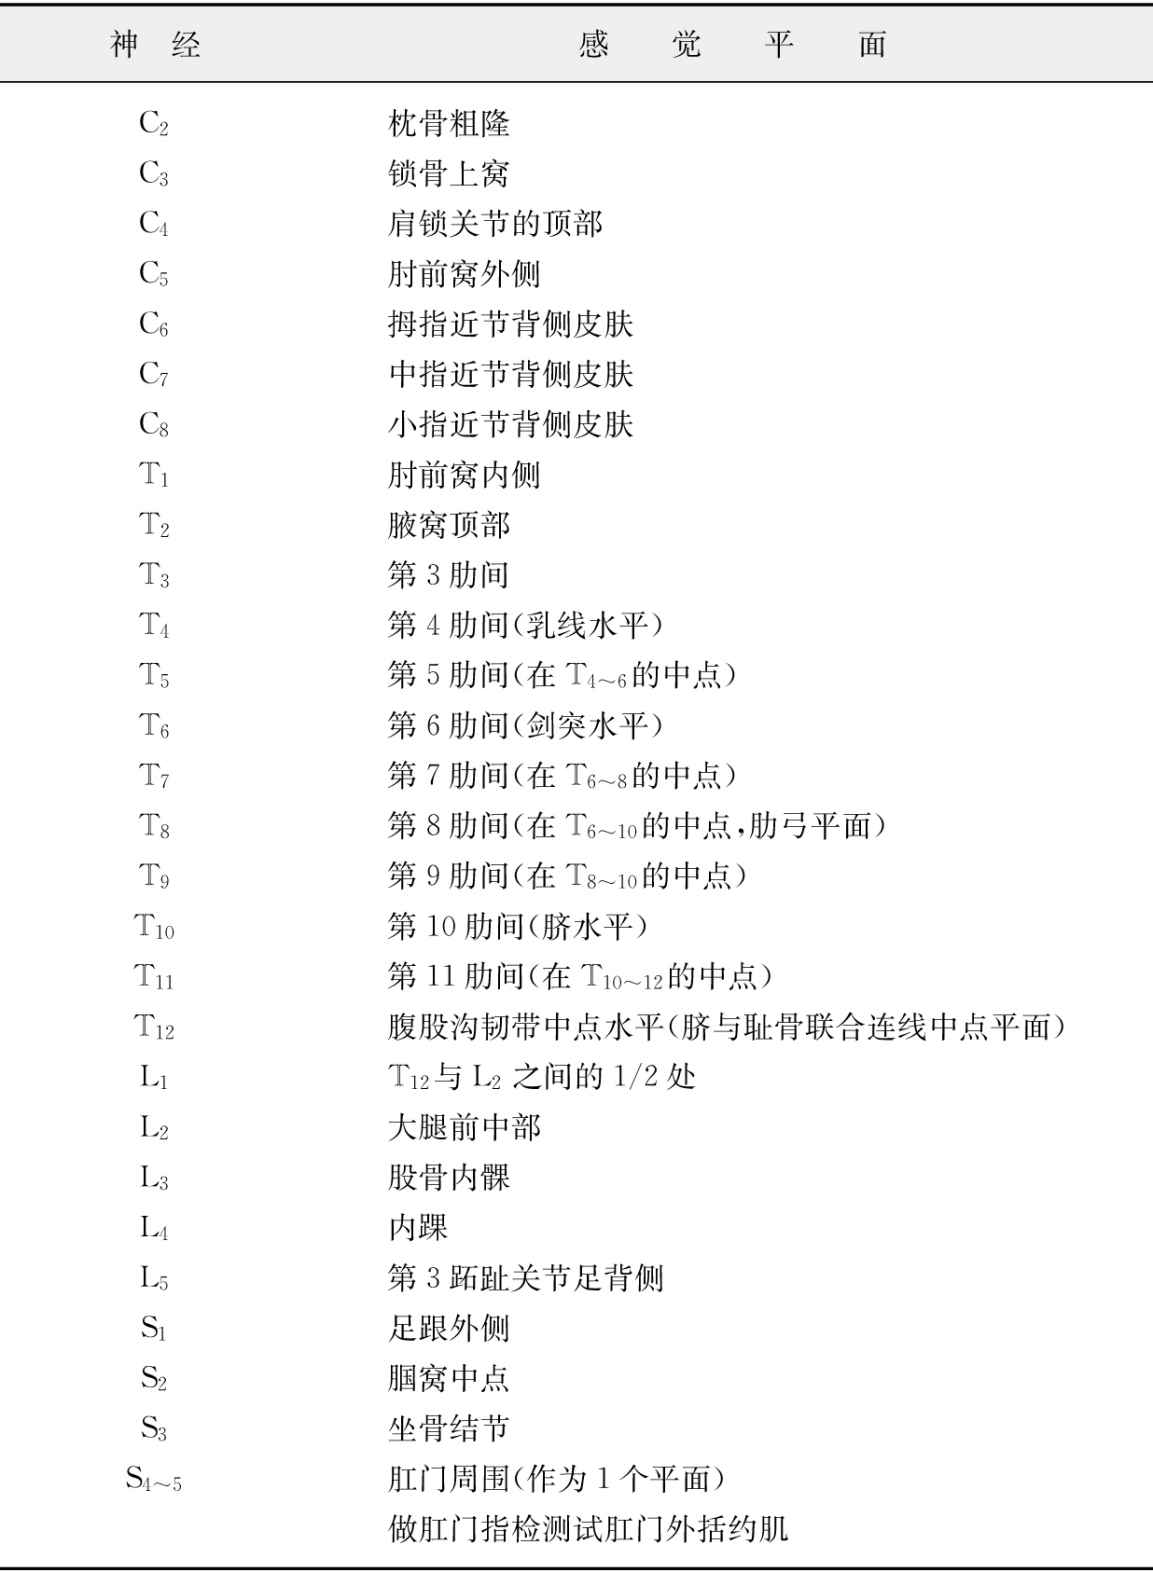
\includegraphics{./images/Image00143.jpg}
\end{table}

运动系统检查(motor
examination)的必查项目为检查身体两侧10对肌节关键肌,左右侧各选一块关键肌。检查顺序为从上而下,肌力分为6级,分别用0~5级来表示:0级=完全瘫痪;1级=肌肉可收缩,但不能产生动作;2级=肢体能在床面上移动,但不能抬起;3级=肢体能抵抗重力离开床面,但不能抵抗阻力;4级=肢体能做抗阻力运动,但不完全;5级=正常肌力。

另外还需要评估肌张力情况,肌张力增高为肌肉松弛状态下的紧张度和被动运动时的阻力增高,可分为:①痉挛性肌张力增高------上肢屈肌、下肢伸肌,见于上运动神经元病变(锥体束损害);②强直性肌张力增高------铅管样或齿轮样,见于锥体外系病变。肌张力降低见于下运动神经元损害、小脑、后索、肌病。

脊髓运动平面评估见表\ref{tab18-4}。

\begin{table}[htbp]
\centering
\caption{运动平面评估}
\label{tab18-4}
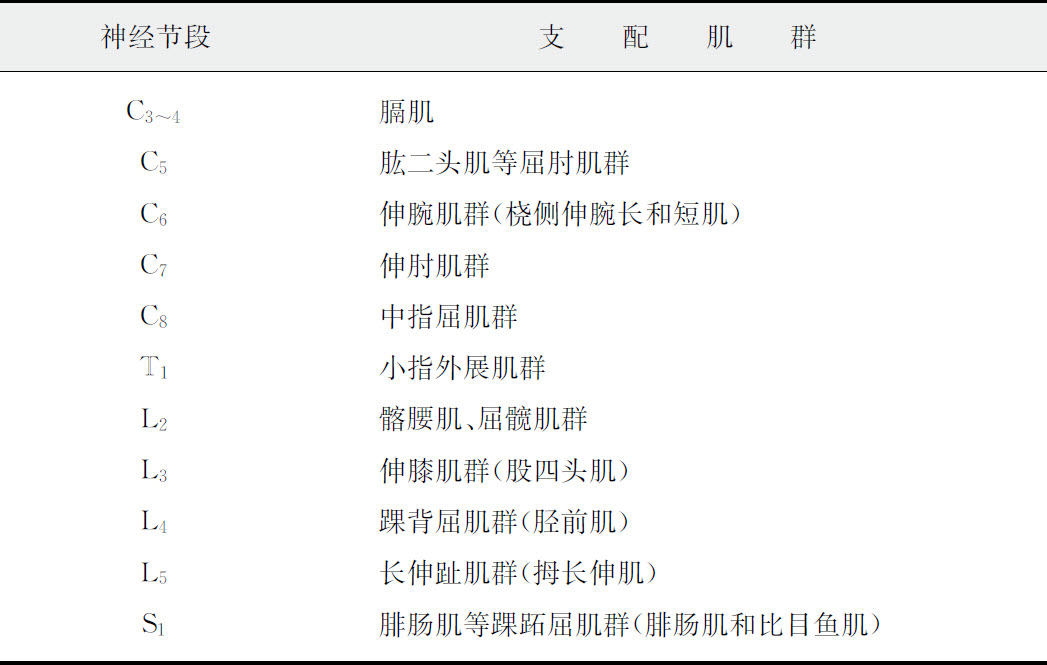
\includegraphics{./images/Image00144.jpg}
\end{table}

除对以上这些肌肉进行两侧检查外,还要检查肛门外括约肌,以肛门指检来评估感觉括约肌收缩,评定分级为存在或缺失(即在患者总表上填有或无)。如果存在肛门括约肌自主收缩,则运动损伤为不完全性。

\subsubsection{脊髓损伤如何早期诊断?应做哪些辅助检查?}

有严重外伤史,早期急救就应想到是否有脊髓损伤,注意急救和搬运方法,使患者脊柱保持正常生理曲线,防止加重损伤。

如患者局部疼痛,有运动、感觉、反射及括约肌和自主神经功能障碍,即可考虑脊髓损伤,同时根据感觉运动平面判断神经损伤节段。根据临床体征及X线、CT、MRI等辅助检查结果可确诊。

脊髓损伤的辅助检查有X线、CT、MRI、体感诱发电位、脊髓造影等检查。

(1)X线 常规摄脊柱正侧位片、必要时照斜位片。阅片时测量椎体前部和后部的高度与上下邻椎相比较;测量椎弓根间距和椎体宽度;测量棘突间距及椎间盘间隙宽度并与上下邻近椎间隙相比较。测量正侧位上椎弓根高度。X线片基本可确定骨折部位及类型。

(2)CT 有利于判定移位骨折块侵犯椎管程度和发现突入椎管的骨块、组织或椎间盘。

(3)MRI 对判定脊髓损伤状况极有价值。MRI可显示脊髓损伤早期的水肿、出血,并可显示脊髓损伤的各种病理变化,脊髓受压、脊髓横断、脊髓不完全性损伤、脊髓萎缩或囊性变等。

(4)体感诱发电位和运动诱发电位 体感诱发电位是测定躯体感觉系统(以脊髓后索为主)传导功能的检测法。对判定脊髓损伤程度有一定帮助,但只能反映上行传导通路的功能状态。运动诱导电位是于大脑皮层运动区(如手区或脚区)的部位给予磁刺激,激发大脑的运动神经径路而引起的手或脚部肌肉的动作电位,可用于评估脊髓受损程度,反映运动神经径路的功能状态。

(5)脊髓造影 对陈旧性外伤性椎管狭窄诊断有意义。

\subsubsection{脊髓损伤后残损神经功能判断标准是什么?}

美国脊髓损伤协会(American Spinal Injury
Association,ASIA)与国际脊髓学会(International Spinal Cord
Society,ISCoS)联合制订的国际标准,即为脊髓损伤神经学分类国际标准(International
Standards for the Neurological Classification of Spinal Cord
Injury,ISNCSCI)(2006),是评价脊髓损伤患者运动和感觉功能损害的临床标准,分为五级。

A级 完全性损伤:S\textsubscript{4~5} 节段无感觉和运动功能保留。

B级 不完全性损伤:在神经平面以下(包括S\textsubscript{4~5}
节段)保留感觉功能,但无运动功能。

C级 不完全性损伤:在神经平面以下保留运动功能,且神经平面以下至少一半关键肌肌力<3级。

D级 不完全性损伤:在神经平面以下保留运动功能,且神经平面以下至少一半关键肌肌力≥3级。

E级 正常:感觉及运动功能正常。

当一个患者被评为C或D级时,必须是不完全性伤,即在骶段S\textsubscript{4~5}
有感觉或运动功能存留。此外,该患者必须具备如下两者之一:①肛门括约肌有自主收缩;②运动平面以下有3个节段以上有运动功能保留。

另外,美国脊髓损伤协会于2009年1月发表了自主神经功能评定标准,该标准包括解剖学诊断,一般自主神经功能评定,下尿道、直肠、性功能,尿流动力学评定四部分。

\subsubsection{脊柱脊髓损伤患者应怎样搬运和急救?}

凡疑有脊柱骨折者,应使患者脊柱保持正常生理曲线。切忌使脊柱做过伸、过屈的搬运动作,应使脊柱在无旋转外力的情况下,3人用手同时平抬平放至木板上,人少时可用滚动法。

对疑有颈椎损伤的患者,要有专人扶托下颌和枕骨,沿纵轴略加牵引力,使颈部保持中立位,患者置木板上后用沙袋或折好的衣物放在头颈的两侧,防止头部转动,并保持呼吸道通畅。

脊柱脊髓伤有时合并严重的颅脑损伤、胸部或腹部脏器损伤、四肢血管伤,危及患者生命安全时应首先抢救。

明确诊断的脊髓损伤可立即行甲基强的松龙冲击治疗,国外已将激素冲击治疗延伸到院前急救中,以期减轻脊髓的继发性损伤,促进神经功能的恢复。如可能,应争取早期手术减压和恢复脊柱的稳定性;如病情不允许,可待病情稳定后再行减压固定手术。

\subsubsection{脊髓损伤激素冲击治疗的指征是什么?剂量如何?}

甲基强的松龙是唯一被证实具有减轻急性脊髓损伤继发损伤的糖皮质激素,可改善脊髓血流量,减少脂质过氧化,稳定细胞膜的离子通道,促进钙离子外移,减少细胞内钙超载,提高神经元的兴奋性和传导性,抑制儿茶酚胺的代谢与积聚等。

明确诊断脊髓损伤8小时内的患者应立即给予甲基强的松龙冲击治疗,首先15~30mg/kg于15分钟内静脉推注,45分钟后给予每小时5.4mg/kg持续静脉泵入,在损伤3小时以内接受甲基强的松龙治疗时,应维持治疗24小时;在损伤后3~8小时开始的,如无复杂的内科疾病,应接受甲基强的松龙维持治疗48小时
\protect\hyperlink{text00024.htmlux5cux23ch42-23}{\textsuperscript{{[}42{]}}}
。美国3次大规模的多中心研究表明,甲基强的松龙可减轻脊髓损伤的继发性损害,促进脊髓神经功能的恢复,并不明显增加感染和消化道出血的发生率。受伤8小时后给予甲基强的松龙治疗无明显益处,而并发症有所增加,因此不建议使用。

\subsubsection{脊髓损伤治疗措施有哪些?}

明确诊断的脊髓损伤可立即行甲基强的松龙冲击治疗。脊髓损伤的功能恢复主要取决于脊髓损伤程度,故及早解除对脊髓的压迫是保证脊髓功能恢复的首要问题。手术治疗是对脊髓损伤患者全面康复治疗的重要部分。手术目的是恢复脊柱正常轴线,恢复椎管内径,直接或间接地解除骨折块或脱位对脊髓神经根的压迫,稳定脊柱(通过内固定加融合),其手术方法包括前路和后路减压+融合+内固定术,可根据患者和医师的情况具体选择融合方法和内固定材料。颈椎现多采用前路手术,胸腰椎可采用后路或前路手术。

其他综合疗法包括:①脱水疗法,应用20%甘露醇250ml,2次/天,目的是减轻脊髓水肿;②自由基清除剂,如维生素E、A、C及辅酶Q等,钙通道阻滞剂、利多卡因等的应用被认为对防止脊髓损伤后的继发损害有一定好处;③促进神经功能恢复的药物,如三磷酸胞苷二钠和维生素B\textsubscript{1}
、B\textsubscript{6} 、B\textsubscript{12}
等;④支持疗法,注意维持患者的水和电解质平衡,注意热量、营养和维生素的补充;⑤早期康复锻炼。

近年来,随着分子生物学技术及干细胞研究的深入,基因治疗及细胞移植技术在实验室已取得可喜的进展。有学者将神经营养因子(NT-3)基因导入骨髓基质干细胞,通过基因转移和细胞移植从而加强神经生长因子的表达,促进受损神经纤维再生,并且在远端形成更多的突触连接,提高了脊髓损伤修复水平。亦有学者强调早期控制脊髓的炎症反应,减轻脊髓的继发性损害,进而保护脊髓功能。

脊髓损伤尤其是高位脊髓损伤易发生下述并发症:①呼吸衰竭和呼吸道感染;②褥疮;③泌尿系统感染;④自主神经系统功能紊乱如体温失调;⑤便秘等。应给予积极防治。

\subsubsection{脊髓损伤预后如何?}

脊髓损伤的预后与损伤部位及严重程度相关。颈髓如颈1、2完全横断性损伤,患者多因呼吸衰竭立即死亡,如能及时气管插管辅助呼吸,可能挽救生命,但高位截瘫,自主呼吸能力差,并发症多,预后不良;颈3、4、5的损伤由于影响到膈神经,未及时治疗患者也常早期因呼吸衰竭死亡。随着医疗水平和院前急救的发展,送达医院则多能存活,因呼吸功能受到影响,较易出现肺部感染等并发症;下颈髓损伤患者,随着手术及内固定技术、重症医学科监护治疗、综合治疗和康复治疗水平明显提高,早期病死率已明显下降,功能恢复与脊髓损伤程度和病理改变有关。胸腰段脊髓损伤常遗留感觉运动等功能障碍。

脊髓损伤治疗费用高,大多遗留不同程度的功能障碍,患者丧失工作能力,生活质量下降,后续治疗仍需大量费用,给家庭和社会带来沉重的负担。目前仍需积极探索脊髓损伤治疗手段,以求改善脊髓损伤患者的预后。

\subsection{腹腔间隔室综合征和骨筋膜室综合征}

\subsubsection{什么是腹腔间隔室综合征?哪些疾病可导致腹腔间隔室综合征?}

腹腔间隔室综合征(abdominal compartment
syndrome)是指4~6小时内3次准确的测量腹内压,其最小值>20mmHg和(或)6小时内两次测量腹腔灌注压<50mmHg,或腹腔内出现新的脏器功能障碍。

腹内压即腹腔内的压力,正常腹内压为0~5mmHg,腹腔灌注压即腹腔内脏器的灌注压=平均动脉压-腹内压。腹腔内高压(intra-abdominal
hypertension)是指4~6小时内3次准确的测量腹内压其最小值>12mmHg和(或)6小时内两次测量腹腔灌注压<60mmHg。腹内高压根据腹腔内压力可分为四级:Ⅰ级12~15mmHg;Ⅱ级16~20mmHg;Ⅲ级21~25mmHg;Ⅳ级>25mmHg。

根据发病原因可分为原发性、继发性腹腔间隔室综合征。原发性腹腔间隔室综合征常常为腹腔或盆腔损伤或手术所致,如严重腹部创伤手术或损伤控制手术、腹膜炎、急性重症胰腺炎、骨盆骨折、腹膜后血肿、肝移植术后等;继发性腹腔间隔室综合征为腹外原因所致的腹内压增高,常见于严重感染、烧伤、毛细血管渗漏、大量液体复苏等。有研究报道,在综合性重症医学科连续收治的256例患者中,内科患者、择期手术、急症手术和创伤患者分别占46.8%、27.9%、16.6%和8.7%,28天内32.1%的患者发生腹腔内高压,4.2%的患者发生腹腔间隔室综合征。

\subsubsection{腹腔间隔室综合征的治疗措施有哪些?}

腹腔间隔室综合征可引起的严重病理生理改变,包括胃肠道和肝脏血流减少、功能障碍,胸腔容量和肺顺应性下降,回心血量减少,心输出量降低,血压下降,肾脏灌注不足,肾功能不全,颅内血流减少,腹壁血流减少等,病情发展可迅速导致多器官功能障碍综合征,因此一旦确诊须积极处理
\protect\hyperlink{text00024.htmlux5cux23ch22-23}{\textsuperscript{{[}22{]}}}
。

腹腔间隔室综合征的治疗可分为非手术和手术治疗方法
\protect\hyperlink{text00024.htmlux5cux23ch19-23}{\textsuperscript{{[}19{]}}}
。非手术治疗包括积极控制原发病,镇静,半卧位体位,胃肠减压,使用呋塞米(速尿)或白蛋白加呋塞米脱水,应用胃肠动力药物,保持肠道通畅,避免过度复苏,连续肾脏替代治疗等。手术腹腔减压是治疗腹腔高压综合征的有效手段,但手术指征尚存在争议。有学者认为当腹内压>20mmHg时即应行手术减压。但也有学者认为外科减压的指征不一定是这些监测指标,只要患者出现明显病理生理损害就应该手术减压。现大多采用开腹手术,延迟闭合伤口或使用各种人工材料暂时关闭伤口,后期手术修复。

\subsubsection{什么是骨筋膜室综合征,如何诊断?}

骨筋膜室综合征(limb compartment
syndrome)指四肢密闭的骨筋膜室内压力骤然升高,使血流量大幅度减少甚至中断,而导致受累组织坏死的临床综合征
\protect\hyperlink{text00024.htmlux5cux23ch23-23}{\textsuperscript{{[}23{]}}}
。肢体遭受外伤、外界压迫、缺血再灌注、筋膜室容积减小等损伤后,组织水肿可使筋膜室内的压力升高,首先阻碍毛细血管静脉回流,继而因微小动脉受压引起肌肉和神经缺血性坏死。

受伤肢体局部肿胀是最明显的局部体征:患处疼痛,牵拉患肢和所累及的肌肉时有剧痛;局部张力升高伴有肿胀,并在短时间内不断加重,皮色苍白,不能扪及动脉搏动,感觉异常;晚期患肢出现典型的5P征------疼痛(pain)、感觉异常(paresthesia)、苍白(pallor)、肢体瘫痪(paralysis)和脉搏消失(pulseless)。X线摄片和多普勒检查可以帮助明确病因,骨筋膜室内压力的测定有助于明确病情程度。

如有发生骨筋膜室综合征的原发疾病存在,就要考虑到此疾病发生可能,伤后要密切关注肢体肿胀情况、皮肤颜色、远端血运和感觉运动情况。一旦出现典型的症状和体征,诊断不难。但处理已较困难,关键是早期诊断和早期治疗。正常的骨筋膜间室压力为0~15mmHg,当压力达到20~30mmHg时,疼痛和感觉异常会出现,当压力达到30~40mmHg时,如不及时降低室内压,肌肉神经将发生缺血性坏死。此时骨筋膜间室压力尚未到患者的动脉舒张压,因此远端动脉搏动仍然存在,所以不能以远端动脉搏动情况来判断肢体是否已出现严重缺血。最直观的做法是用压力测定仪测定各筋膜室压力。

\subsubsection{骨筋膜室综合征如何处理?}

骨筋膜室综合征影响预后的关键是诊断和治疗的时机,如能及时做出正确的诊断,早期综合治疗可能避免手术。如病情持续进展,即应尽早及时切开减压治疗。血管源性本征预后较差;不能及时治疗的病例将造成肢体的不可逆损伤残疾,甚至威胁患者的生命。因此,一旦确诊为骨筋膜室综合征,就必须立即行筋膜切开术,同时积极治疗原发病。对将发生骨筋膜室综合征的患肢抬高,并不能增加筋膜间室内的血流。

综合治疗措施包括以下几个方面:①去除一切增加骨筋膜室压力的因素,如去除石膏、放松绷带等;②输注高渗液体缓解室内组织水肿,甘露醇为首选,可以有效地减少渗出,促进渗出液的回吸收,从而降低骨筋膜室内压力,甘露醇还是氧自由基的清除剂,可减轻缺血后水肿和肌肉坏死;③使用碱性液体,纠正酸中毒和高钾血症;另外,碱化尿液可防治大量肌红蛋白阻塞肾小管,预防肾衰竭;有肾衰竭者应及时行肾脏替代治疗;④高压氧有减轻水肿和减少肌肉坏死的作用,其作用机制可能是氧供应增加后使血管收缩,从而降低毛细血管中的压力,减少渗出液和漏出液;文献报道经高压氧处理者,伤口愈合较好,可减少组织坏死;⑤并发症的治疗,包括抗感染、神经营养药物、镇痛以及防治高钾、肾衰竭、休克等。

如果患者伤肢持续性疼痛并进行性加重、高度肿胀、骨筋膜室压力增高、患肢被动牵拉引起损伤局部肌肉疼痛剧烈、有一定的神经功能障碍体征,就要警惕病情的变化,及时测定骨筋膜室压力,一般具有上述症状,再加上骨筋膜室室内压力达到30~40mmHg或距动脉舒张压仅20~30mmHg,就具备手术指征。手术治疗方法主要为骨筋膜室切开减压术,现在多主张做长切口、多室切开,以达到充分减压的目的。

\subsection{胸部创伤}

\subsubsection{胸部多发性肋骨骨折如何处理?}

肋骨参与构成胸廓,起着保护胸腹腔器官的作用,而一旦肋骨损伤即可导致胸廓完整性改变,影响器官功能。肋骨骨折在胸部创伤中很常见,约占90%,2根或2根以上的肋骨骨折称为多发性肋骨骨折。多发性肋骨骨折由于损伤大、创伤严重、并发症多、复合伤发生率高,导致救治难度加大,已经引起重视。大量研究发现,多发性肋骨骨折多由直接暴力所致,巨大暴力作用于肋骨时可能导致多发性肋骨骨折,而残余暴力则可使肋骨骨折端移位而引发血、气胸、血气胸、胸腹脏器损伤,故肋骨骨折易导致内脏器官损伤,应避免漏诊,尤其多发性肋骨骨折一旦出现则应及时检查和处理。

(1)综合治疗 多发性肋骨骨折一般仅需用肋骨固定带或胸带固定即可,但应积极处理并发症,尤其是危及患者生命的创伤。具体措施包括:①保持呼吸道通畅;②开放性气胸需清创缝合,尽快使其转为闭合性,并进行闭式引流;③血气胸有呼吸困难者应早期行胸腔闭式引流术;④连枷胸或浮动胸壁患者,应选择合适的外固定或内固定方法固定胸壁;⑤如出现呼吸困难、低氧血症,应尽早气管插管或气管切开,行机械通气治疗,选择适当的呼气末正压,并间断性肺复张治疗(手法或机械通气),促进膨胀不全的肺复张,以纠正低氧血症;⑥经验性应用抗生素,强化气道管理,防止继发性肺部感染。

(2)镇痛 肋骨骨折疼痛剧烈,一般在24~48小时内明显,且限制了患者的胸壁活动,可增加患者肺部感染概率、干扰呼吸功能及骨折恢复,影响患者的病情、住院时间及病程和转归。有效地控制疼痛是多发性肋骨骨折治疗的关键之一。目前临床中较多使用镇痛药物干预治疗,也可采用局部封闭、肋间神经阻滞、硬膜外阻滞和镇痛药等方法。近年来,皮下电刺激镇痛用于肋骨骨折也收到良好的镇痛效果。最近Davies等
\protect\hyperlink{text00024.htmlux5cux23ch43-23}{\textsuperscript{{[}43{]}}}
报道,持续胸椎旁阻滞镇痛效果与持续硬膜外镇痛效果相仿,且镇痛失败、低血压、呕吐、尿潴留等并发症发生率明显低于后者,该治疗方法已经逐步得到认可。

(3)手术治疗 多发性肋骨骨折出现下列情况时需手术治疗:①合并胸腔内脏器损伤,属于开胸手术指征,肋骨骨折复位内固定仅作为一种附加手术,这类胸内损伤包括:持续性胸腔出血;经胸腔引流后仍持续性大量漏气、呼吸窘迫;心血管损伤;开放性肋骨骨折;胸腹腔内脏破裂;创伤性膈疝。②连枷胸或浮动胸壁患者,需行手术治疗,以使肋骨复位内固定、稳定胸壁。在胸部创伤中严重胸壁软化时出现反常呼吸,进一步发展时会出现严重的呼吸功能不全,甚至ARDS。手术内固定是稳定胸壁、消除反常呼吸的重要环节,也避免了软化区胸壁对深部肺组织的进一步挫伤。固定方法可采用钢丝、克氏针、接骨板及钢板内固定等。

\subsubsection{何谓张力性气胸?如何处理?}

张力性气胸是严重的胸部创伤的一种类型,常见于胸部穿透伤或较大而深的肺裂伤、支气管或食管破裂。裂口与胸膜腔以活瓣的形式相通,吸气时活瓣开放,空气进入胸膜腔;呼气时活瓣关闭,气体不能自胸膜腔排除,致胸腔内气体不断增加,压力逐渐增高。伤侧肺萎陷,纵隔移向健侧、严重影响呼吸功能,产生低氧血症。同时由于胸腔内负压消失,纵隔内大血管扭曲,回心静脉血流受阻,心输出量减少,使患者迅速出现呼吸循环衰竭而危及患者生命。

如果胸部创伤的患者出现进行性加重的呼吸困难,一侧呼吸音明显减弱或消失,颈静脉怒张,器官明显移向对侧,应考虑张力性气胸。特别值得注意的是,不应等待胸部X线的结果,而应立即行胸腔穿刺或胸腔闭式引流,以免耽误抢救时间。

张力性气胸病情紧急需立即急救,可即刻使用粗针头穿刺胸膜腔减压,并外接单向活瓣装置,如在针尾缚一顶端开口的乳胶手指套,进一步处理应安置胸腔闭式引流并连接负压吸引装置,以利加快气体排出,促进肺复张。

\subsubsection{何谓外伤性血胸?应如何处理?}

胸部创伤后引起胸膜腔积血称为外伤性血胸,是胸部创伤的严重并发症之一。胸腔内大出血是胸部创伤早期的主要死亡原因之一,血胸的血液可来自:①肺组织裂伤出血;②肋间血管或胸廓内动脉破损出血:③心脏、大血管破裂出血;④膈肌破裂同时伴有肝、脾破裂出血。血液又是细菌良好的培养基,一旦感染即容易合并脓胸,需要引起重视。

外伤性血胸主要危害在于急性失血及胸膜腔积血压迫肺组织、使纵隔移位等。出血量、出血速度与症状轻重、病情严重程度密切相关。

治疗原则:①非进行性血胸应根据积血量的多少,采用胸腔穿刺或闭式胸腔引流术,并合理使用抗生素预防感染。②进行性血胸在输血、补液抗休克的同时及时行开胸探查术。③凝固性血胸待伤情稳定后尽早手术,清除血块。④感染性血胸应给予抗感染,胸腔穿刺、胸腔闭式引流术,必要时早期扩清术排除脓液,并积极全身支持治疗。

\subsubsection{严重胸部外伤急诊开胸手术的指征有哪些?}

严重胸部创伤是严重创伤患者的重要死亡原因之一,占所有创伤患者死亡率的25%~50%,急诊开胸手术是威胁生命的严重胸部创伤早期救治和复苏的重要治疗手段。现在普遍认为,单纯锐器伤所致的心脏骤停、心脏损伤、心包填塞、大量空气栓塞以及胸腔内大量出血,应立即开胸手术。阻断降主动脉、控制膈下大出血,保证心脑灌注也是急诊开胸的指征
\protect\hyperlink{text00024.htmlux5cux23ch44-23}{\textsuperscript{{[}44{]}}}
。具体适应证、禁忌证见表\ref{tab18-5}。

\begin{table}[htbp]
\centering
\caption{胸部外伤急诊开胸手术的适应证、禁忌证}
\label{tab18-5}
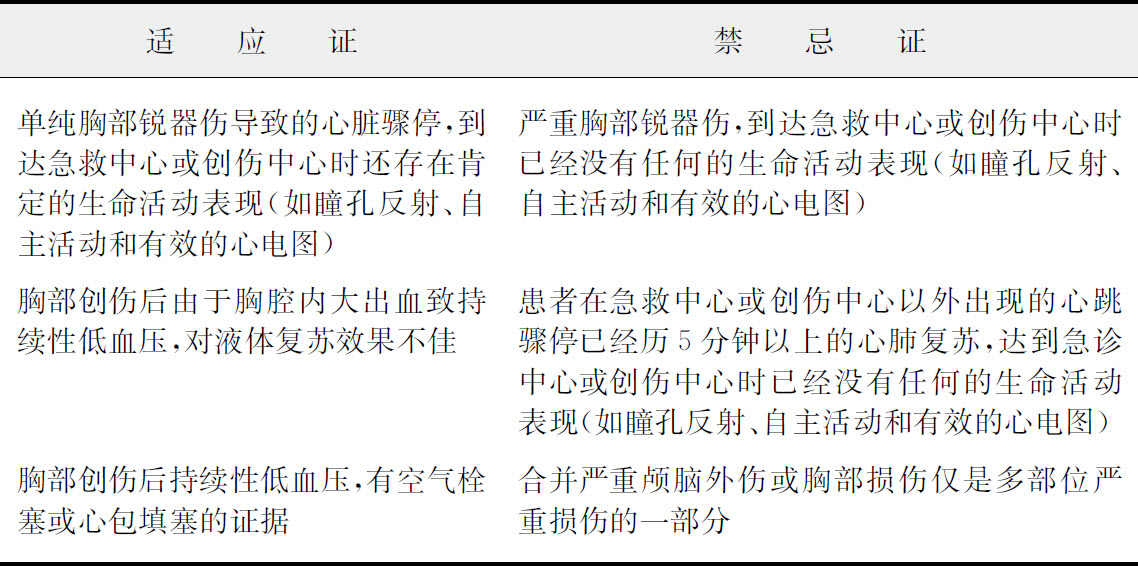
\includegraphics{./images/Image00145.jpg}
\end{table}

\subsubsection{创伤相关的心脏骤停患者,开胸心脏胸内复苏的成功率如何?}

开胸手术胸内心脏按压复苏成功的关键在于早期的认识、及时诊断以及迅速积极的干预和治疗。胸部钝器伤心脏骤停患者扩容的同时应立即急诊开胸手术,进行胸内心脏按摩、解除心包填塞、修补心脏和大血管损伤、控制胸腔内和外出血。2001年美国外科医师学院创伤委员会发表一篇荟萃分析,收录了自1996年至1999年的42篇相关研究,研究对象为急救中心进行开胸手术治疗的创伤相关的心脏骤停患者,共7000余例入组。研究结果表明,胸部锐器伤患者开胸手术抢救的存活率为11%(4482例,存活500例)。开胸手术治疗对于即将到达或发生在急救中心的单纯锐器伤导致的心脏骤停确实能挽救生命,但对于在院外发生的钝器创伤所致的心脏骤停或合并严重胸外损伤的患者(如严重颅脑外伤和脊柱外伤),开胸心脏按压并不改变预后。

\subsubsection{骨盆骨折的类型有哪些?}

骨盆骨折是一种严重外伤,多由暴力直接挤压骨盆所致。骨盆骨折多为高能量创伤,多见于交通事故、塌方、施工事故和火器伤。骨盆骨折常伴有致命性大出血,半数以上伴有合并症或多发性创伤,可以导致创伤性失血性休克及合并损伤盆腔脏器。临床上应尽早稳定骨折,减少骨盆再移位和再损伤,控制出血,稳定血流动力学,缩短抢救复苏期,提高生存率。既往多采用保守治疗,如骨牵引、骨盆悬吊、石膏固定等方法,导致畸形愈合、创伤性关节炎等后遗症的发生率明显升高。近年来,随着对骨盆骨折认识的深入,主张对不稳定性骨盆骨折采取更加积极的治疗方法,如外固定架固定、切开复位内固定等,从而降低病死率和致残率,Simonian等
\protect\hyperlink{text00024.htmlux5cux23ch45-23}{\textsuperscript{{[}45{]}}}
报道,创伤早期应用外固定术,致命性失血性休克的复苏成功率从22%降到8%。

骨盆骨折的分类有很多种,以往据部位分为:①撕脱性骨折;②骨盆环的孤立性骨折;③骨盆环的双骨折或骨折脱位(完整性完全丧失,可能发生环的各种程度变化);④骶、尾骨骨折;⑤髋臼骨折合并股骨头中心性脱位。目前得到公认的分类有Tile和Young-Burgess分类系统(见表\ref{tab18-6}及表\ref{tab18-7})。Tile分类依据骨折稳定性、暴力方向和性质将骨盆环损伤分为A、B、C三型;依据暴力的传递途径及骨折发生的先后顺序,Young-Burgess将骨盆骨折分为前后压缩(anterior
posterior compression)、侧方压缩(lateral
compression)、垂直剪切(vertical
shear)和混合性损伤挤压和(或)压缩4种。

\begin{table}[htbp]
\centering
\caption{Tile分类}
\label{tab18-6}
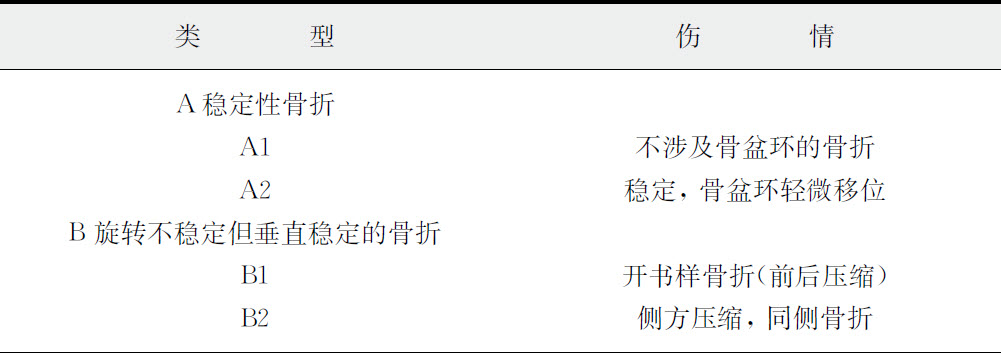
\includegraphics{./images/Image00146.jpg}
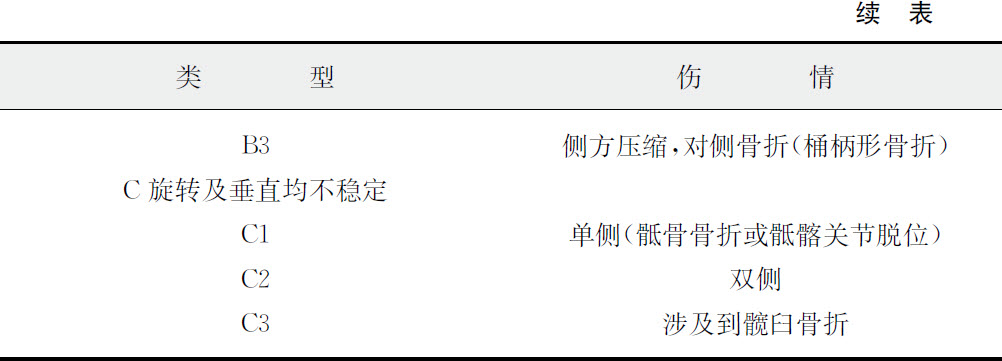
\includegraphics{./images/Image00147.jpg}
\end{table}

\begin{table}[htbp]
\centering
\caption{Young-Burgess分类}
\label{tab18-7}
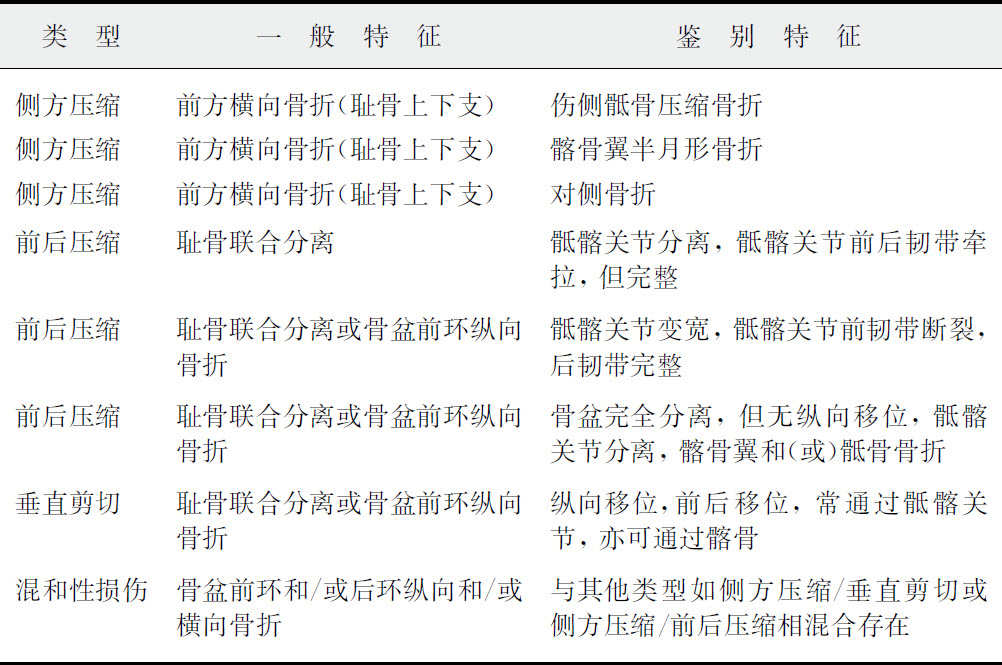
\includegraphics{./images/Image00148.jpg}
\end{table}

\subsubsection{骨盆骨折应进行哪些影像学检查,有何临床意义?}

X线检查是骨盆骨折诊断和指导治疗的重要依据。X线检查应包括3个标准的骨盆像:①前后位,能显示骨盆骨折的基本征象;②入口位;③出口位。骨盆位片和出入口斜位片对骨盆前环损伤诊断的相对敏感性为75%,但对后环的漏诊率却达47%。

在骨盆骨折的整体显像方面,CT扫描不如X线检查理想,但能较好显示局部微小损伤,相对敏感性为86%,而联合X线诊断相对敏感性可达96%。近年来,随着影像学技术和设备的发展,多排螺旋CT、三维重建技术越来越多地应用于骨盆骨折的诊断和治疗方案的确立。特别是螺旋CT联合三维重建技术的联合应用可快速、准确、清晰、立体、全面地显示骨折线的走向和骨折端的移位,无须特殊体位,最大限度地减少了患者的痛苦及检查过程中的相关并发症。

MRI检查可显示骨盆内脏器损伤情况,但检查时间长,临床应用受到一定的限制。旋转数字成像、同位素扫描在骨盆骨折检查中也可以作为选择,但检查影响因素较多,临床应用较少。

骨盆骨折患者在行影像学检查搬运过程中,应注意保持骨盆的稳定性,可采用骨盆兜或大的被单等将骨盆简单外固定,防止在搬运过程中骨折断端活动而加重组织损伤。

\subsubsection{骨盆骨折的急救治疗原则是什么?}

(1)评估 快速进行全身评估,确定呼吸道是否通畅,呼吸是否正常,有无合并其他部位的严重致命性创伤,并进行相应的监测和处理。

(2)补液 开放足够的补液通道,最好建立在上肢或颈部,快速补充血容量,纠正休克,稳定循环功能。骨盆骨折的失血量极大,若经积极大量输血等抢救措施后休克仍未能纠正,可考虑结扎一侧或两侧髂内动脉,或经导管行髂内动脉栓塞术。

(3)止血 腹腔检查怀疑出血者应及时用外固定器暂时固定骨盆,并紧急开腹探查止血;若腹腔检查未发现出血征象,应行血管造影以便发现出血点,及时进行栓塞止血。若考虑腹膜后血肿,怀疑为静脉或骨折端出血,切勿切开后腹膜,以避免出血难以控制。

(4)止痛 骨盆骨折常会引起患者剧烈疼痛,因此减少对患者的搬动以及分散其注意力,必要时则给予止痛药物(须在明确无颅脑和胸部外伤后方可给药)。

(5)开放性伤口的处理 清洁伤口的处理可一期清创缝合,臀部会阴的伤口易被粪便污染,应局部清创引流。

(6)固定 骨折的整复和固定是控制和预防骨盆出血的重要方法,急诊行外固定支架固定后可减少骨折出血发生,有利于纠正休克。

(7)转运 全身情况稳定后须对骨盆骨折进行局部固定,对不稳定的骨盆骨折,可暂时用外固定架固定,及时转运至相关治疗机构。

\subsubsection{骨盆骨折的局部治疗原则是什么?}

骨盆骨折首先进行抢救治疗,遵循生命第一的原则。全身情况稳定后对骨盆骨折进行详细的影像学检查,并对骨折类型、稳定性、移位以及患者状态进行评价,依据骨折类型采取相应的治疗方案。

A型骨盆骨折:骨盆环稳定,骨折无移位时卧床采用保守治疗。

B型骨盆骨折:骨盆旋转不稳定,可行闭合复位外固定或切开复位内固定。

C型骨盆骨折:骨盆旋转和垂直方向均不稳定时一般要根据骨折部位决定。骨折线通过骶髂关节应采用切开复位内固定;骨折线在骶髂关节外通过髂棘或骶骨时,若未合并其他损伤时则采用闭合复位外固定;若复位不满意,则采用切开复位内固定。

外固定方法多指采用外固定架固定,通过髂嵴前半向髂翼内置入直径5mm螺纹钉4~8枚,间隔距离1cm以上,通过牵引或手法复位后用外固定支架与两侧的螺纹钉连接,达到外固定的目的。适合于不稳定性骨盆骨折需要进行紧急抢救或转运的患者。

内固定术应在病情稳定后进行,一般在伤后5~7天进行,最迟不超过两周,一旦骨折3周以上,那么损伤将难以整复。手术方法根据骨折部位、骨折移位情况及骨盆稳定情况进行选择。

复杂C型骨盆骨折常伴有盆腔脏器的损伤,如直肠、膀胱、尿道及阴道损伤,亦可合并其他部位的骨折和软组织损伤,因此已经成为创伤骨科的难点,临床可以采用经皮空心拉力螺钉
\protect\hyperlink{text00024.htmlux5cux23ch46-23}{\textsuperscript{{[}46{]}}}
结合外固定架的微创技术,能在一定程度上减少创伤、降低感染概率、降低骨折愈合干扰,且固定牢固。在四川汶川“5.12”特大地震中有相当一部分骨盆骨折患者使用了该新技术,收到很好的疗效。

\subsubsection{骨盆骨折的并发症有哪些?}

骨盆是全身力量传递的枢纽,血液供应丰富,其内容纳人体重要脏器,解剖结构复杂。骨盆骨折常伴有严重并发症,而且常较骨折本身更为严重。因此,治疗时应先考虑全身情况,优先处理危及生命的并发症。

(1)失血性休克和后腹膜血肿 骨盆各骨主要为松质骨,盆壁肌肉多,临近又有许多动、静脉丛,血液供应丰富,盆腔与后腹膜间隙系疏松结缔组织构成,有巨大腔隙可容纳出血,因此骨折后常可引起广泛出血致失血性休克,其发生率可高达15%~50%,患者亦可出现腹胀、腹痛、肠鸣音减弱或腹肌紧张等腹膜刺激征的症状。为了与腹腔内出血鉴别,可行诊断性腹腔穿刺,但穿刺不要过深,以免进入腹膜后血肿内,临床必须严密观察,反复检查。

腹膜后血肿是骨盆骨折常见的并发症,巨大腹膜后血肿可蔓延到肾区、膈下或肠系膜,可能继发感染,或者腹腔内压力增高,形成腹腔间室综合征,甚至继发急性肾衰竭。因此,对腹膜后出血者应严密观察,进行输血、输液。若经积极的抗休克治疗无好转,则须立即行介入治疗,选择性栓塞单侧或两侧髂内动脉。一旦出现腹腔间室综合征,则可行开腹减压,有利于肾脏等器官功能的恢复,但不建议手术清除腹膜后血肿,以免出现无法逆转的大出血。

(2)尿道或膀胱损伤 对骨盆骨折的患者应考虑是否存在尿路损伤以及膀胱损伤,前者多见。双侧耻骨支骨折及耻骨联合分离多可引起尿道膜部继发性损伤,患者可出现排尿困难、尿道口溢血等表现。对尿道断裂者宜先放置导尿管,导尿有困难时可行耻骨上膀胱造瘘及尿道会师术,后期再行尿道扩张术以纠正尿道狭窄,而膀胱破裂者则可行耻骨上膀胱造瘘术或修补术。

(3)肠道损伤 骨盆骨折伴有阴部开放性损伤时多可合并直肠损伤,发生率为1.25%~6%
\protect\hyperlink{text00024.htmlux5cux23ch47-23}{\textsuperscript{{[}47{]}}}
。直肠破裂如发生在腹膜反折以上,可引起弥漫性腹膜炎;如发生在其以下则可发生直肠周围感染,故直肠损伤者应立即行剖腹探查及结肠造瘘,术后应充分引流。

肠嵌顿是骨盆骨折的一种少见并发症
\protect\hyperlink{text00024.htmlux5cux23ch48-23}{\textsuperscript{{[}48{]}}}
。如早期未能发现将造成肠坏死、肠穿孔、严重腹腔感染等严重后果,故对于骨盆骨折后腹胀明显的患者均应保持高度警惕。一经诊断,应急诊行剖腹探查。

(4)神经损伤 多在骶骨骨折时发生,其中腰骶神经干的骶1及骶2最易受损伤,可出现臀肌、腘绳肌和小腿腓肠肌肌群的肌力减弱,小腿后方及足外侧部分感觉丧失。骶神经损伤严重时可出现跟腱反射消失,但很少出现括约肌功能障碍。目前多认为神经损伤治疗效果不佳,故而采用保守治疗,预后与神经原发损害程度有关。若神经损伤轻微,则预后好,一般1年内可望恢复。

(5)其他少见并发症 股动脉损伤、臀上动脉损伤、腹膜后感染、假性动脉瘤、脂肪栓塞综合征、创伤性膈疝等,发生率低。诊治的关键是保持足够的警惕性,多观察体征变化。

\begin{center}\rule{0.5\linewidth}{\linethickness}\end{center}

参考文献

\protect\hyperlink{text00024.htmlux5cux23ch1-23-back}{{[}1{]}} .Mock
C,Quansah R,Krishnan R,Arreola-Risa C,Rivara F.Strengthening the
prevention and care of injuries
worldwide.Lancet.2004.363(9427):2172-2179.

\protect\hyperlink{text00024.htmlux5cux23ch2-23-back}{{[}2{]}}
.杨自力,吴恒义.多发伤及其急救.创伤外科杂志.2004.6(1):75-77.

\protect\hyperlink{text00024.htmlux5cux23ch3-23-back}{{[}3{]}}
.贾健,金鸿宾,王基.多发伤的特征及其对策探讨.创伤外科杂志.2000.2(1):23.

\protect\hyperlink{text00024.htmlux5cux23ch4-23-back}{{[}4{]}}
.Holtslag HR,van BEF,Lindeman E,Leenen LP.Determinants of long-term
functional consequences after major trauma.J
Trauma.2007.62(4):919-927.

\protect\hyperlink{text00024.htmlux5cux23ch5-23-back}{{[}5{]}}
.刘中民.改善急救模式 提高创伤救治水平.中华急诊医学杂志.2002.12(02):79-80.

\protect\hyperlink{text00024.htmlux5cux23ch6-23-back}{{[}6{]}} .Keel
M,Trentz O.Pathophysiology of
polytrauma.Injury.2005.36(6):691-709.

\protect\hyperlink{text00024.htmlux5cux23ch7-23-back}{{[}7{]}} .Hill
AG,Hill GL.Metabolic response to severe injury.Br J
Surg.1998.85(7):884-890.

\protect\hyperlink{text00024.htmlux5cux23ch8-23-back}{{[}8{]}}
.Hietbrink F,Koenderman L,Rijkers G,Leenen L.Trauma:the role of
the innate immune system.World J Emerg Surg.2006.1:15.

\protect\hyperlink{text00024.htmlux5cux23ch9-23-back}{{[}9{]}} .Levy
RM,Mollen KP,Prince JM,et al.Systemic inflammation and remote organ
injury following trauma require HMGB1.Am J Physiol Regul Integr Comp
Physiol.2007.293(4):R1538-1544.

\protect\hyperlink{text00024.htmlux5cux23ch10-23-back}{{[}10{]}}
.Bianchi ME.DAMPs,PAMPs and alarmins:all we need to know about
danger.J Leukoc Biol.2007.81(1):1-5.

\protect\hyperlink{text00024.htmlux5cux23ch11-23-back}{{[}11{]}} .Pugin
J.Dear SIRS,the concept of“alarmins”makes a lot of sense.Intensive
Care Med.2008.34(2):218-221.

\protect\hyperlink{text00024.htmlux5cux23ch12-23-back}{{[}12{]}} .Lenz
A,Franklin GA,Cheadle WG.Systemic inflammation after
trauma.Injury.2007.38(12):1336-1345.

\protect\hyperlink{text00024.htmlux5cux23ch13-23-back}{{[}13{]}}
.Giannoudis PV,Harwood PJ,Loughenbury P,Van Griensven M,Krettek
C,Pape HC.Correlation between IL-6 levels and the systemic
inflammatory response score:can an IL-6 cutoff predict a SIRS state.J
Trauma.2008.65(3):646-652.

\protect\hyperlink{text00024.htmlux5cux23ch14-23-back}{{[}14{]}}
.DeLong WG Jr,Born CT.Cytokines in patients with polytrauma.Clin
Orthop Relat Res.2004.42(2):57-65.

\protect\hyperlink{text00024.htmlux5cux23ch15-23-back}{{[}15{]}}
.Choudhry MA,Bland KI,Chaudry IH.Trauma and immune response---
effect of gender differences.Injury.2007.38(12):1382-1391.

\protect\hyperlink{text00024.htmlux5cux23ch16-23-back}{{[}16{]}}
.Bogner V,Kirchhoff C,Baker HV,et al.Gene expression profiles are
influenced by ISS,MOF,and clinical outcome in multiple injured
patients:a genome-wide comparative analysis.Langenbecks Arch
Surg.2007.392(3):255-265.

\protect\hyperlink{text00024.htmlux5cux23ch17-23-back}{{[}17{]}}
.Morley JR,Smith RM,Pape HC,MacDonald DA,Trejdosiewitz
LK,Giannoudis PV.Stimulation of the local femoral inflammatory
response to fracture and intramedullary reaming:a preliminary study of
the source of the second hit phenomenon.J Bone Joint Surg
Br.2008.90(3):393-399.

\protect\hyperlink{text00024.htmlux5cux23ch18-23-back}{{[}18{]}}
.Deitch EA,Xu D,Kaise VL.Role of the gut in the development of
injury-and shock induced SIRS and MODS:the gut-lymph hypothesis,a
review.Front Biosci.2006.11:520-528.

\protect\hyperlink{text00024.htmlux5cux23ch19-23-back}{{[}19{]}}
.Franke A,Lante W,Kollig E,Koeller M,Schinkel C,Markewitz
A.Exogenous IL-12 and its effect on TH1/TH2 cell activity after cardiac
surgery.Shock.2009.32(4):366-373.

\protect\hyperlink{text00024.htmlux5cux23ch20-23-back}{{[}20{]}}
.Miller AC,Rashid RM,Elamin EM.The“T”in trauma:the helper T-cell
response and the role of immunomodulation in trauma and burn patients.J
Trauma.2007.63(6):1407-1417.

\protect\hyperlink{text00024.htmlux5cux23ch21-23-back}{{[}21{]}} .Brohi
K,Singh J,Heron M,Coats T.Acute traumatic coagulopathy.J
Trauma.2003.54(6):1127-1130.

\protect\hyperlink{text00024.htmlux5cux23ch22-23-back}{{[}22{]}}
.Gebhard F,Huber-Lang M.Polytrauma --- pathophysiology and management
principles.Langenbecks Arch Surg.2008.393(6):825-831.

\protect\hyperlink{text00024.htmlux5cux23ch23-23-back}{{[}23{]}}
.曹同瓦.多发性损伤的急诊处理原则.中华急诊医学杂志.2005.16(10):86-88.

\protect\hyperlink{text00024.htmlux5cux23ch24-23-back}{{[}24{]}}
.黎沾良.多发性创伤的救治策略.临床外科杂志.2005.24(06):329-330.

\protect\hyperlink{text00024.htmlux5cux23ch25-23-back}{{[}25{]}}
.邓勇,韩庆,白卫东.创伤急救模式对救治水平的影响.中华创伤杂志.2004.13(11):46-48.

\protect\hyperlink{text00024.htmlux5cux23ch26-23-back}{{[}26{]}} .Roy
JW,Graham MC,Griffin AM,Gainer JL.A novel fluid resuscitation
therapy for hemorrhagic shock.Shock.1998.10(3):213-217.

\protect\hyperlink{text00024.htmlux5cux23ch27-23-back}{{[}27{]}} .Nolan
J.Fluid resuscitation for the trauma
patient.Resuscitation.2001.48(1):57-69.

\protect\hyperlink{text00024.htmlux5cux23ch28-23-back}{{[}28{]}}
.Soreide E,Deakin CD.Pre-hospital fluid therapy in the critically
injured patient --- a clinical
update.Injury.2005.36(9):1001-1010.

\protect\hyperlink{text00024.htmlux5cux23ch29-23-back}{{[}29{]}}
.Bickell WH,Wall MJ Jr,Pepe PE,et al.Immediate versus delayed fluid
resuscitation for hypotensive patients with penetrating torso
injuries.N Engl J Med.1994.331(17):1105-1109.

\protect\hyperlink{text00024.htmlux5cux23ch30-23-back}{{[}30{]}}
.Finfer S,Bellomo R,Boyce N,French J,Myburgh J,Norton R.A
comparison of albumin and saline for fluid resuscitation in the
intensive care unit.N Engl J Med.2004.350(22):2247-2256.

\protect\hyperlink{text00024.htmlux5cux23ch31-23-back}{{[}31{]}}
.吴岳嵩.多发伤的早期处理.中华创伤杂志.1997.5(01):66-67.

\protect\hyperlink{text00024.htmlux5cux23ch32-23-back}{{[}32{]}}
.Burris D,Rhee P,Kaufmann C,et al.Controlled resuscitation for
uncontrolled hemorrhagic shock.J Trauma.1999.46(2):216-223.

\protect\hyperlink{text00024.htmlux5cux23ch33-23-back}{{[}33{]}} .Stone
HH,Strom PR,Mullins RJ.Management of the major coagulopathy with
onset during laparotomy.Ann Surg.1983.197(5):532-535.

\protect\hyperlink{text00024.htmlux5cux23ch34-23-back}{{[}34{]}}
.Johnson JW,Gracias VH,Schwab CW,et al.Evolution in damage control
for exsanguinating penetrating abdominal injury.J
Trauma.2001.51(2):261-269;discussion 269-271.

\protect\hyperlink{text00024.htmlux5cux23ch35-23-back}{{[}35{]}} .Pape
HC,Hildebrand F,Pertschy S,et al.Changes in the management of
femoral shaft fractures in polytrauma patients:from early total care to
damage control orthopedic surgery.J
Trauma.2002.53(3):452-461;discussion 461-462.

\protect\hyperlink{text00024.htmlux5cux23ch36-23-back}{{[}36{]}}
.徐姜定.颅内压增高监测及治疗进展.浙江临床医学.2003.6(07):481-482.

\protect\hyperlink{text00024.htmlux5cux23ch37-23-back}{{[}37{]}}
.Myburgh J,Cooper DJ,Finfer S,et al.Saline or albumin for fluid
resuscitation in patients with traumatic brain injury.N Engl J
Med.2007.357(9):874-884.

\protect\hyperlink{text00024.htmlux5cux23ch38-23-back}{{[}38{]}}
.Roberts I,Yates D,Sandercock P,et al.Effect of intravenous
corticosteroids on death within 14 days in 10008 adults with clinically
significant head injury(MRC CRASH trial):randomised
placebo-controlled trial.Lancet.2004.364(9442):1321-1328.

\protect\hyperlink{text00024.htmlux5cux23ch39-23-back}{{[}39{]}}
.Edwards P,Arango M,Balica L,et al.Final results of MRC CRASH,a
randomised placebo-controlled trial of intravenous corticosteroid in
adults with head injury-outcomes at 6
months.Lancet.2005.365(9475):1957-1959.

\protect\hyperlink{text00024.htmlux5cux23ch40-23-back}{{[}40{]}}
.Roquilly A,Mahe PJ,Seguin P,et al.Hydrocortisone therapy for
patients with multiple trauma:the randomized controlled HYPOLYTE
study.JAMA.2011.305(12):1201-1209.

\protect\hyperlink{text00024.htmlux5cux23ch41-23-back}{{[}41{]}}
.江基尧.客观分析颅脑创伤患者国际多中心循证医学研究结论.中华创伤杂志.2009.25(8):673-674.

\protect\hyperlink{text00024.htmlux5cux23ch42-23-back}{{[}42{]}}
.Bracken MB,Shepard MJ,Holford TR,et al.Administration of
methylprednisolone for 24 or 48 hours or tirilazad mesylate for 48 hours
in the treatment of acute spinal cord injury.Results of the Third
National Acute Spinal Cord Injury Randomized Controlled Trial.National
Acute Spinal Cord Injury Study.JAMA.1997.277(20):1597-1604.

\protect\hyperlink{text00024.htmlux5cux23ch43-23-back}{{[}43{]}}
.Davies RG,Myles PS,Graham JM.A comparison of the analgesic efficacy
and side effects of paravertebral vs epidural blockade for thoraotomy a
systematic review and metaanalysis of randomized trials[J].Br J
Anaesth,2006,96(4):418.

\protect\hyperlink{text00024.htmlux5cux23ch44-23-back}{{[}44{]}} .Hunt
PA,Greaves I,Owens WA.Emergency thoracotomy in thoracic trauma-a
review.Injury,2006,37:1-19.

\protect\hyperlink{text00024.htmlux5cux23ch45-23-back}{{[}45{]}}
.Simonian PT,Routt ML Jr,Harrington RM,et al.Anterior versus
posterior provisional fixation in the unstable pelvis.A biomechanical
comparison[J].Clin Orthop,1995,(310):245.

\protect\hyperlink{text00024.htmlux5cux23ch46-23-back}{{[}46{]}}
.丁浩,马金忠.不稳定型骨盆骨折的手术治疗.中国骨与关节损伤杂志,2007,22(1):50.

\protect\hyperlink{text00024.htmlux5cux23ch47-23-back}{{[}47{]}} .Mason
WTM,Khan SN,James CL,et al.Complications of temporary and definitive
external fixation of pelvic ring
injuries[J].Injury,2005,36(5):599-604.

\protect\hyperlink{text00024.htmlux5cux23ch48-23-back}{{[}48{]}}
.Stubbart JR,Merkley M,Bowel entrapment within pelvic
fractures:acase report and review of the lit erature J Orthop
Trauma,1999,13(2):145.

\protect\hypertarget{text00025.html}{}{}

